\documentclass[11pt,journal]{IEEEtran}
%\usepackage{hyperref}
%\usepackage[breaklinks]{hyperref}
\usepackage{tikz}
\usetikzlibrary{arrows,automata,calc,shapes}
\usepackage{breakurl}
\usepackage{url}
\usepackage{amsfonts}
\usepackage{amsmath}
\usepackage{amssymb}
\usepackage{listings}
\usepackage{array}
% Set listings to use small monospaced font.
\lstset{basicstyle=\small\ttfamily,tabsize=4}
\usepackage{graphicx}
\usepackage{booktabs}
\ifCLASSOPTIONcompsoc
% IEEE Computer Society needs nocompress option
% requires cite.sty v4.0 or later (November 2003)
\usepackage[nocompress]{cite}

\else
% normal IEEE
\usepackage{cite}
\fi
\setcounter{tocdepth}{2}
\hyphenation{op-tical net-works semi-conduc-tor}


\begin{document}
	\title{Exploring the limitations of the Atelier B automated prover}
	
	\author{Agata~Borkowska,~UID: 1690550,~\IEEEmembership{MSc in Computer Science,~University of Warwick}\\Supervisor: Jane Sinclair}
	% The paper headers

	\markboth{}%
	{ \MakeLowercase{\textit{}}: }
	
	\IEEEcompsoctitleabstractindextext{%
		\begin{abstract}
			%\boldmath
			Atelier B is a tool for formal software development through refinement, using the B method. It incorporates an automated and an interactive prover, which has been recognized as the most thorough prover for B theory. It aided with numerous industrial projects and has been used as a basis for many other tools. Nevertheless it has multiple shortcomings. Various approaches have been suggested and taken to improve its performance, including extensions to the proof rule base, plug-ins and third-party software. 
			
			At the same time researchers and engineers who are new to formal methods, often struggle to even get familiar with the tool on its own, as its output may lack clarity at times and overall be not very user-friendly. Thus they get discouraged quickly, and lose interest in formal methods.
			
			In this work we strive to provide new users with practical guidelines on how to understand the feedback given by the Atelier B provers and how to reduce the number of proof obligations which are not demonstrated automatically, since manually discharging them is the most time-consuming part of the proof process\cite{survey}. The secondary goal isto establish the limitations of the prover without such additions, and discover at which point they become necessary.  
	\end{abstract}
	\begin{IEEEkeywords}
		B method, formal verification, specification, abstract machine, proof, system development
	\end{IEEEkeywords}}
	% IEEEtran.cls defaults to using nonbold math in the Abstract.
	% This preserves the distinction between vectors and scalars. However,
	% if the journal you are submitting to favors bold math in the abstract,
	% then you can use LaTeX's standard command \boldmath at the very start
	% of the abstract to achieve this. Many IEEE journals frown on math
	% in the abstract anyway. In particular, the Computer Society does
	% not want either math or citations to appear in the abstract.
	
	% Note that keywords are not normally used for peerreview papers.
	
	% make the title area
	\maketitle
	
	
	% To allow for easy dual compilation without having to reenter the
	% abstract/keywords data, the \IEEEcompsoctitleabstractindextext text will
	% not be used in maketitle, but will appear (i.e., to be "transported")
	% here as \IEEEdisplaynotcompsoctitleabstractindextext when compsoc mode
	% is not selected <OR> if conference mode is selected - because compsoc
	% conference papers position the abstract like regular (non-compsoc)
	% papers do!
	\IEEEdisplaynotcompsoctitleabstractindextext
	% \IEEEdisplaynotcompsoctitleabstractindextext has no effect when using
	% compsoc under a non-conference mode.
	
	
	% For peer review papers, you can put extra information on the cover
	% page as needed:
	% \ifCLASSOPTIONpeerreview
	% \begin{center} \bfseries EDICS Category: 3-BBND \end{center}
	% \fi
	%
	% For peerreview papers, this IEEEtran command inserts a page break and
	% creates the second title. It will be ignored for other modes.
	\IEEEpeerreviewmaketitle
	
	\tableofcontents
	\clearpage
	\section{Introduction}
	\IEEEPARstart{T}{he} aim of formal specification and verification is to ensure the correctness of software. While overall less popular than quality assurance through testing, it is primarily, but not exclusively used in safety-critical areas, where thorough testing may not feasible or may be very costly. It also aids with writing consistent documentation and guiding the development process. As such, it is of interest not just to academics, but to people working in industry as well. 
	
	However in our colleagues' and our own experience, the tools used for this purpose sometimes have rather scant documentation and are generally not user-friendly. The error messages they output are difficult to understand, rarely point the user at what to do next. There is not much of a community developed around this area, which would welcome beginners who often need pointers that may seem obvious to anyone more experienced.
	
	When a new user, who is just learning how to apply formal methods, has to struggle with both understanding the theory and the intricacies of the tools, they may easily get discouraged. This project is aimed exactly at new users who are at loss and do not know how to interpret the behaviour of the tools. We aim to give them guidelines on how to approach proofs, as well as warnings about certain behaviours which may not be in line with standard logic or set theory.
	
	We believe that popularizing the interest in formal methods will help diminish their reputation of being inaccessible and requiring long and expensive training, before they can be applied in industry. Seeing as others have also begun to notice that such statements no longer hold\cite{amazon}, we approach the topic with hope that this trend will continue in the years to come.
	
	We choose to work with the B method, which has been developed over 20 years ago by J.-R. Abrial. Since then it has become a significant element in safety assurance, especially in the railway industry. Furthermore, we chose Atelier B software, developed by ClearSy Ltd., as the most widely accredited, although far from perfect. It has contributed to multiple industrial projects, as well as being used for teaching formal methods at university level. Thus our work may be of interest to both engineers and academics.

	\subsection{Project Structure}% Tell the reader a little about the project. (Ideally, just go through the ToC and write a little prose on each entry)
	
	\subsection{The B method}
	The B method is based on logic and set theory, and at least some prior knowledge of these two areas is very helpful when starting to work with it. However we will still go over basic concepts and definitions, as well as define notation used throughout this project, to avoid ambiguities.
	
	The development process in the B method begins with formalising a given specification as an abstract machine, using the B language. This stage will be the focus of our work. The abstract machine can be viewed as a state machine. Its state is described by the values of the variables, and it is taken from one state to another by operations which change those values. 
	
	It has to be stressed that at this stage, there is no notion of sequencing or temporal logic. An operation performs all its actions simultaneously, in parallel. For the same reason, loops cannot exist in an abstract machine, and recursion or an operation making a call to another one, is not permitted. On the other hand, there are many features which help with expressing a specification with clarity. At the abstract machine stage, a user can employ set comprehension, summation, and similar operations. All of them are easy to express in the B syntax.
	
	Another feature available there is nondeterminism. It is not considered erroneous to ask for any random element of a set to be assigned to a variable. However, at the later stages of the development, the level of nondeterminism must decrease, until it is completely removed when the model is ready to be implemented.
	
	One might ask why nondeterminism should be used at all, if it is only going to be erased. It allows the user to focus on other details, and not be distracted by the specifics at a given moment. It makes it easier to inspect other behaviours of the machine, while the user does not care what value some of the variables have. Overall, it serves to narrow down the user's concerns.
	
	Once the abstract machine has been written, the user ascertains that the specification has been formalised correctly, and proceeds with the development. The next stage is to refine the abstract machine step by step, to reduce nondeterminism, and to turn set operations into ones which programmers are more familiar with. Moving from one step to another, requires the user to verify that all properties of the machine, as defined at the very beginning, are preserved.
	
	The whole process ends at the implementation stage, where all data structures and the values of the variables are concrete. Sets are now replaced with arrays, and loops can be used. Additionally, the user can include standard library machines in the project. From this point, code can be generated, to some extent automatically.
	
	\subsection{Structure of an abstract machine}
	In the B language, using Atelier B syntax, an abstract machine usually has the following clauses, in order:
	\begin{itemize}
		\item machine name - must match the name of the file, followed by a list of parameters without type definitions, given in brackets as a comma-separated list, for example \texttt{Bagmch(ITEMS, max\_elem)}.
		\item \texttt{SETS} - deferred sets, i.e. those which will be specified at a later point. They can be used to define types of constants and variables.
		\item \texttt{CONSTANTS} - either scalar or set-valued constant are declared here.
		\item \texttt{PROPERTIES} - types of constants and the relations between them. 
		\item \texttt{DEFINITIONS} - constants with a concrete value. According to the \emph{Interactive Prover Reference Manual}, it is preferable to define such constants here, rather than declare them in the Constants clause and assign them a value in the Properties clause, because it reduces the amount of rewriting the tool does.\cite{Prover guide} 
		\item \texttt{VARIABLES} - declarations of variables, which the machine operates on.
		\item \texttt{INVARIANT} - properties of the machine that have to be maintain at every point of its operation. This clause includes type definitions of the variables, bounds on their values, and relations between them and the constants.
		\item \texttt{ASSERTIONS} - a series of statements which can act as intermediate steps in a proof. Note that they are necessarily ordered and every statement is proven under the assumption of those preceding it.
		\item \texttt{INITIALISATION} - the initial state of the machine, where the values of the variables are assigned.
		\item \texttt{OPERATIONS} - operations performed on the variables of the machine. Some of them may change the values of the variables, while other may only output a result of some calculation.
	\end{itemize}

	The first few clauses up to and including Assertions are considered the static part of the machine, and they provide definitions or describe properties that hold at all times. The last two clauses, namely Initialisation and Operations, form the dynamic part of the machine, as they either assign or change values of the variables.
	
	Many of the clauses are optional, for example Definitions or Assertions. Others are closely linked together. For example it is imperative to declare Properties, if the machine contains a Constants clause. Similarly, if there is a Variables clause, it must be followed by Initialisation. Such dependencies are picked by static analysis in the source code editor.
	
	Other clauses which are not analysed in this project, are structuring clauses, such as \texttt{USES}, \texttt{SEES}, or \texttt{INCLUDES}, and clauses necessary for refinement and implementation.
	
	\subsection{Atelier B Provers}
	Beyond serving as a source code editor for the B method, Atelier B also allows the users to verify the machines they have written and check that they are indeed correct. This is done in three ways. 
	
	As could be expected, static analysis takes place while the user is writing the code, and serves to indicate primarily syntax errors. It may also come in useful when a user mistakenly calls a set operation on a scalar value or vice versa.  
	
	Once the machine is free from these errors, the user may proceed to generate proof obligations. They are statements which should be demonstrated to hold, or as it is sometimes called, discharged, or else the machine is likely to be incorrect. It should be noted that a proof obligation may be demonstrated to hold, be it by the tools included in the software or others, or manually, but it may not be disproved. The problem is known to be undecidable.[CITE] Therefore an undischarged proof obligation does not necessarily point to a mistake in the machine, but quite possibly is a result of a shortcoming of the prover tool.
	
	Proof obligations generated by Atelier B can be divided into two types. Most proof obligations will be concerned with preservation of the Invariant by the Initialisation and the Operations which change the variables. A proof obligation of this type, which cannot be demonstrated, indicates that performing an operation may result in the machine entering an invalid state.
	
	The second kind of proof obligations check the well-defineness property of certain expressions. A proof obligation of this kind which is impossible to discharge indicates that the user has likely not been specific enough when defining variables and their properties. For example, the expression $max(\varnothing)$ is erroneous, because there is no greatest element in the empty set. Similarly in the B language, for a set $A$, the expression $card(A)$ makes sense if and only if $A$ is finite. The well-defineness conditions for all such expressions can be found in the \emph{B Language Reference Manual}\cite{b reference}.
	
	With the proof obligations generated, the user may begin the process of discharging them. Atelier B includes two provers which can achieve this. Firstly, the Automatic Prover should be used to demonstrate as many proof obligations as possible without the user's input.
	
	If that is not sufficient, the user may employ the Interactive Prover. In it, they may view the undischarged proof obligations and guide the proof process along, for example by suggesting intermediate steps of the proof. The Interactive Prover also allows users to search through the proof rule base included in the software, as well as enables users to write their own proof rules.
	
	Finally it is worth mentioning that the Atelier B provers' work by rule inference, and for a proof to succeed, the rules have to be ordered correctly for all the goals to be demonstrated. It has its limitations, and one attempt to mitigate them is to employ the predicate prover, included in the Interactive Prover's for the user to call. The predicate prover transforms the proof into quantified statements and attempts proof by contradiction.	
	
	\section{Definitions and Conventions}
	
	\subsection{Definitions and notations}
	Care shall be taken to use unambiguous notation and terms. We begin with a brief summary of the logic notation, comparing it to the B syntax, which comprises of ASCII characters or approximations thereof. We first give the unicode symbol which will be used when discussing logical expressions in this writeup, followed by the ASCII equivalent written in a monotype font, as it can be seen in code snippets. 
	\begin{itemize}
		\item AND is denoted by $\wedge$ or \texttt{\&}
		\item OR is denoted by $\vee$ or \texttt{or}
		\item the existential quantifier is $\exists$ or \texttt{\#}
		\item the universal quantifier is $\forall$ or \texttt{!}
		\item the negation is denoted by $\neg$ or \texttt{not(x)}
	\end{itemize}
	This list includes only the most commonly seen symbols, some of which may not be intuitive to some users. Other symbols will be defined if or when they are needed.
	
	Since the B method is heavily based on Zermelo-Fraenkel set theory, it is worth recalling key concepts and definitions from this area.\cite{Goldrei}
	
	Firstly, a \textbf{set} is a collection of distinct objects, which we will call \textbf{elements}. We say that $a$ is an element of a set $x$ or that it belongs to the set $x$. Set membership is a binary relation denoted with the symbol '$\in$' or with '\texttt{:}' in the B syntax.
	
	By the Axiom of Extensionality, two sets are equal if and only if they have the same elements. Hence, in set axiomatic set theory $\{x\} = \{x, x\}$ - for each element of the first set is in the second, and each $x$ in the second set is in the first one. The B method also recognizes this equality\cite{b-method}. 
	
	Note that a set can be an element of another set, however a set must not belong to itself - i.e. there does not exist a set $x$ such that $x \in x$. This is known as Russell's Paradox.
	
	By the Null Set Axiom, there exists a set having no elements - i.e. the \textbf{empty set}. It is denoted $\varnothing$ or \texttt{\{\}} in the B syntax. The empty set is unique.
	
	A \textbf{subset} $y$ of a set $x$ is a set such that each element of $y$ is also in $x$, but not necessarily the other way round. It is denoted $y \subseteq x$ or \texttt{y <: x} in the B syntax. Note that the empty set is a subset of every set, and that every set is a subset of itself.
	
	The \textbf{powerset} of a set $x$, denoted $\mathbb{P}(x)$ or \texttt{POW(x)} in the B syntax is the set containing all subsets of the set $x$. For example if $x = \{a,b\}$, then $\mathbb{P}(x) = \{\varnothing, \{a\}, \{b\}, \{a,b\}\}$. Thus the expression $y \subseteq x$ is semantically equivalent to $y \in \mathbb{P}(x)$. 
	
	The \textbf{union} of sets $x$ and $y$ is defined as the set of elements which belong to either $x$ or $y$, i.e. $x \cup y = \{z| z \in x \vee z \in y\}$ and in the B syntax it is written as \verb|x\/y|. The \textbf{intersection} of sets $x$ and $y$ is defined to be the set of all elements which belong to both $x$ and $y$, i.e. $x \cap y = \{z | z \in x \wedge z \in y \}$, which in the B syntax is \verb|x/\y|.

	
	Natural numbers will be often seen in this project. Firstly, and a little informally, the set of natural numbers, denoted $\mathbb{N}$ or \texttt{NAT} in the B syntax, is the set $\{0,1,2, ...\}$. The B syntax also has an abbreviation for the natural numbers excluding 0, i.e. \texttt{NAT1} shall be used to mean $\mathbb{N}-\{0\}$.
	
	The natural numbers give the first discrepancy between the B method and the mathematical theories which it is based on, which we encounter throughout this work. Formally, in axiomatic set theory, the natural numbers are defined as follows:
	
	Let $x^+$ denote the successor set of the set $x$, which is $x^+ = x \cup {x}$. Then $\mathbb{N}$ is the smallest (with respect to the number of elements) set such that $\varnothing \in \mathbb{N}$ and if $x \in \mathbb{N}$ then $x^+ \in \mathbb{N}$.
	
	For simplicity, it is often defined that $\varnothing = 0$, $1 = \{\varnothing \}$, $2 = \{\varnothing , \{\varnothing\} \} = \{0,1\}$, and so on. In set theory, every element of the natural numbers is a set itself. This is not the case in B, and an attempt to talk about an element of an $n \in \mathbb{N}$ gives a type error in Atelier B during static analysis.
	
	To make the distinction clear between integers and sets of integers as defined above, we will use the notation $[n]$ for some $n \in \mathbb{N}$ to indicate the set of all integers smaller than $n$, which is: $[n] = \{0,1, ...,n-1\}$. The B syntax has an abbreviation for it, and $[n]$ can be denoted as \texttt{0..n-1}. More generally, this B notation means a segment of natural numbers - for $m, n \in \mathbb{N}$, \texttt{m..n} $= \{x | x \in \mathbb{N} \wedge m \leq x \wedge x \leq n\}$
	
	A \textbf{Cartesian product} of two sets $X$ and $Y$ is the set of all pairs $\{(a,b) | a \in X \wedge b \in Y  \}$. It is denoted $X \times Y$ or \texttt{x*y}. The pairs, also called \textbf{maplets} are written as \texttt{a~|->~b} in the B syntax. They are the elements of relations, functions, and sequences in the B language, and while we will not go into the details of the notation here.
	
	With the help of those definitions we can finally define a finite set. A \textbf{finite} set is a set $x$ such that there exists a bijection between $x$ and $[n]$ for some $n \in \mathbb{N}$.  The B syntax also provides an abbreviation for the set of all finite subsets of a set $x$. \texttt{FIN(x)} is hence defined to be $\{y| y \in \mathbb{P}(x) \wedge y \text{ is finite} \}$.
	
	Then the \textbf{cardinality} of $x$ is the number of elements in $x$, in this case $n$, and is denoted $|x|$ or \texttt{card(x)} in the B syntax. Note that in the B language, the expression \texttt{card(x)} is well-defined only for finite sets.
	
	\subsection{Naming Conventions}
	Throughout this work we will keep to the following naming conventions.
	
	Variables and constants in the B language are named according to the following rules:
	\begin{itemize}
		\item names of sets, including deferred sets and those given as machine parameters, are written in all capitals. In this text, they will also be written in a monotype font, for example \texttt{ITEMS}.
		\item scalar constants' names shall be written in lower case, in a monotype font, for example \texttt{max\_elem}.
		\item names of variables shall be written in lower case, in a monotype font, and must be at least two characters in length, for example \texttt{aa}.
	\end{itemize}
	Single-character variable names are not allowed in the B-syntax, and so we will avoid them in all contexts. They are reserved for wildcards in user-written proof rules.
	
	Furthermore, file names will be written in italic. In the case of Atelier B machine files, the extensions will be omitted. The files will be named according to the following pattern: \emph{[name of the reference machine]\_[abbreviated description of the variation]}. Machine clause names will be written with the first letter upper case, unless they are part of a code snippet.
	
	\section{Literature review}
	The first text to be mentioned in this section has to be Sekerinski's book entitled \emph{Program Development by Refinement: Case Studies Using the B Method}\cite{Sekerinski}. It is a textbook containing a fair introduction to the B method and practical exercises, with various example machines written out and analysed. It served as a key inspiration for this project, and the methods employed in our work follows closely the idea of inspecting a machine in order to gain deeper understanding of the B method. The examples included in this book revolve around implementations of standard data structures and algorithms, such as operations on linked lists, heaps, and trees. Unfortunately, just as so many other positions, this book focuses heavily on refinement and implementation, while not paying as close attention to abstract machines. Nevertheless it illustrates how thorough explanations of a few chosen examples can be helpful to people learning the B method.
	
	
	
	\subsection{Industrial examples}
	Although this work is aimed at students and researchers, it is necessary to put it into perspective of how formal methods can be used in industry. Looking at the applications of formal methods will serve to demonstrate that this work indeed serves a purpose and that there are users who may want to refer to the discoveries done in this project in order to facilitate their work.
	
	As mentioned in the Introduction, formal methods are primarily used in safety-critical areas, where testing is difficult or insufficient as an evidence of the correctness of the software, while failure can result in injury or loss of life. 
	
	An obvious area where formal methods are applicable is medical software. It has been noticed as early as in 1980s that software controlling medical machines and devices needs to be thoroughly checked. They eye-opening incident involved a malfunctioning radiology machine, which dosed patients with lethal doses of radiation. The occurrences were few and difficult to connect, but after an in-depth investigation were attributed to bugs in the software.\cite{therac} Since then formal methods are encouraged, but not mandated by the standards, including \emph{The FDA Software Validation Regulations}\cite{FDA}. Some argue that it is still not enough, and demand even stricter standards. Discussion of this matter can be found in Vogel's book \emph{Medical Device Software Verification, Validation, and Compliance}\cite{vogel}. Many Companies developing medical software have openly declared that they use formal methods to avoid such tragic events. The most notable among them include GE Healthcare\cite{ge} and Hewlett-Packard's Medical Division\cite{hp}.
	
	More recently, the use of formal methods have been explored in the context of cyber-physical systems, such as pacemakers. \cite{pacemaker_kwiatkowska1} \cite{pacemaker_kwiatkowska2} \cite{pacemaker_kwiatkowska3}
	
	Other industrial examples of formal methods in use include Amazon Web Services, which use highly complex systems.\cite{amazon} The engineers there have observed that human intuition is prone to errors and that formal methods help find subtle bugs, which can be easily overlooked by other means of checking the correctness of the software. They use TLA+, a formal specification language developed by Lamport\cite{TLA}. The Amazon Web Services engineers also acknowledge that formal methods in industry have the reputation for requiring long and expensive training before they can be used with confidence, however they have found this opinion to be false. This may be specific to the method they have chosen, but nevertheless it is encouraging that people are questioning such opinions, and are open to trying out this approach despite them.
		
	In particular, the B method is popular in the railway industry. Their use is supported by standards and regulations which describe the requirements for software controlling signalling, communication and processing.\cite{railway standard}.
	
	A prime example of an application of the B-method is the project launched by Siemens Transportation System in collaboration with ClearSy, to develop a driverless, automated shuttle for the Charles de Gaulle Airport\cite{airport shuttle}. It has operated since 2005 and is highly reliable. Specifically the B method was used as a high-level language, because of it being well-suited for proving properties. They have used Atelier B automated and interactive provers in their work, and found that out of over 43000 proof obligations, 97\% were discharged automatically. The remaining over 1400 proof obligations required the use of the interactive prover. They managed to discharge on average 15 proof obligations in a day, and at this scale it was still a very time-consuming task. 
	
	ClearSy has also participated in other, smaller projects. One of them is the development of the software controlling screen doors on the platforms, to make sure that they open simultaneously with the train doors after it stops. The project was carried out in collaboration with R\'{e}gie Autonome des Transports Parisiens (RATP). It was considered very successful and after eight months of operation and controlling over 96000 train stops they did not find any faults in it.\cite{screen doors}
	
	Less directly applicable, although very interesting is the effort of Reichl \textit{et al.} to model a train station in Event-B, using the Rodin tool\cite{station model}. The software which could be built from this model would route trains and control signalling between tracks and intersections, so that collisions are avoided and a train efficiently progresses towards its destination. The aim of this work is to demonstrate what can be achieved in terms of modelling complex interlocking systems with Event-B, and what are the limitations of such models. Of the latter, the key observation is that all stations are different and require careful changes to the model, the source code for which is available online. Furthermore the authors observe that the tool they have used is not yet industry-ready, and there are some promising alternatives under development. This was a very large-scale model in comparison and the authors may have set the bar too high, given the currently available tools. As we have seen before, direct applications of B method or Event-B tend to focus on smaller systems, such as automated doors on a platform.
	

	This selection of examples suffices to prove that formal methods are still applicable and are of interest not just to academics. 
	
	The scale of these projects is infeasible to simulate in this work, however they give us a good idea of the time cost racked up by proof obligations which are not discharged automatically. Conchon and Iguernlala consider decreasing the number of undemonstrated proof obligations to be a good way of reducing the cost of the whole project\cite{survey}, and indeed the figures given by Badeau and Amelot support this claim. 30\% of the time they have spent on working on the abstract model was devoted to proof\cite{airport shuttle}.
	
	Since this work is meant to aid new users of Atelier B, it was interesting and worthwhile to look at what others consider to be shortcomings of the software. Even the engineers of ClearSy themselves have noted that their documentation was lacking and additional documents were necessary for their collaborators from RATP to fully understand their deliverables\cite{screen doors}. Leuschel \emph{et al.} have openly admitted that they found the feedback provided by the prover to be unhelpful with locating the problem\cite{San Juan metro}. Their experience is in line with our own and that of our colleagues.

	\section{Project overview}
	\subsection{The aims of the project}
	The key aim of this project is to discover the limitations of the Atelier B software. In the previous section, we have mentioned some plugins and extensions to the Atelier B software, which were created in order to improve the functionality. They highlight what other users have found lacking in Atelier B and what they have considered in need of improvement. However none of them demonstrate what can be achieved with the original software alone. Hence we strive to assess at what point Atelier B alone becomes insufficient, and the extensions are necessary to successfully verify a project. 
		
	We intend to explore various ways of expressing a specification in the B language, paying attention to how seemingly equivalent expressions result in different proof obligations being generated by the automated prover, and follow it up by seeking an explanation of the differences using the information contained in the source texts. 
	
	A valid question to ask here is why does the number of proof obligations matter and why would one may want to put in the effort to minimise their number. The examples of applications of the B method discussed in the previous section illustrate the scale of the proofs in industrial projects and serves to show that reducing the number of proof obligations which require user input to discharge, can greatly save man-hours. Of course the difference is not significant in the small examples we provide here or little projects developed for teaching purposes. However we believe it to be a good practice to understand factors that might affect work on large scale projects in an industrial setting.
	
	This approach is often taken by students and academics beginning their work with the B-method and the Atelier B software. They are unlikely to have a thorough knowledge of the intricacies of the B-method as implemented in the Atelier B software, and would attempt to write a machine first, then search the manuals to explain unexpected behaviours of the software. The software itself has been found to be unintuitive and not user-friendly, as noted by\cite{San Juan metro}.
	
	From our experience and observations, new users, especially students, tend to blindly follow methods and patterns which their colleagues have found to be effective, without giving much thought to why this works and if its applicable in their particular situation. This phenomenon has been sometimes described as 'cargo cult' in the programming community\cite{Cargo culting}, and is disapproved off, as it often leads to unnecessary obfuscation of the code and decrease of performance in a program. One of such tips we have come across, which served as an inspiration for this work, was to deal with undischarged proof obligations by putting their goal in the Invariant clause of a machine. While this method was found to be working, there are more effective means of reducing the number of proof obligations generated, and thus the time taken to complete the proof.
	
	We hope to provide the new users with an explanation for the most commonly encountered proof obligations which are not automatically discharged, and persistent patterns among them. Both understanding the information given by the automated prover and avoiding undischarged proof obligations in the first place is of interest.
	
	An extension to this aim is answering the question: at what point is it necessary to add user-created rules in order to facilitate the proofs in the automated prover? It needs to be stressed that adding user-created rules is not advised unless it is absolutely necessary - and every manual as well as the works discussing methods of validating such rules stress this point. The rules then have to be thoroughly verified by means other than Atelier B software, to ensure that they are in fact correct. An error in an added rule would invalidate the entire proof process. Hence we will strive to circumvent obstacles by all means other than adding proof rules, before resorting to it. We hope to gather such advice and guidelines and make it accessible to others, so that they may be dissuaded from unnecessarily adding proof rules in their work. It is possible that adding proof rules to the Atelier B's rule base may be avoided entirely in the scenarios we have chosen, as they are by no means exhaustive; otherwise we will present the rules and their proofs for the use of others who wish to study the B-method.

	The observations arising from our work can be separated into two groups. Firstly there will be points highlighting the intricacies of the B method, which can be reasoned about and explained easily using source texts, primarily Abrial's \emph{The B-book}\cite{b-book} and Schneider's \emph{The B-Method}\cite{b-method}. 
	
	Secondly, there will be disparities between the B method and its implementation in the Atelier B software. Not all of them can be classified as bugs, and some are clearly conscious choices which diverge from the pure theory of the B method. The manuals provided with the software will aid us with comparing the implementation to the theory. They are:
	
	\begin{itemize}
		\item \emph{Atelier B 4.0 User Manual}\cite{user manual}
		\item \emph{B Language Reference Manual}\cite{b reference}
		\item \emph{Proof Obligation Manual}\cite{PO reference}
		\item \emph{Interactive Prover Reference Manual}\cite{Prover guide}
	\end{itemize}
	
	\subsection{The scope of the project}
	This work focused on abstract machines - they are the first step towards a formally verified implementation of a specification, thus making them the foundation of any project developed using the B method. An implication of this choice is focusing on set-related structures, including relations which are understood as sets of maplets, and operations such as set comprehension, union, and intersection. These abstract constructs are not allowed in the later stages of the development, where all data structures have to be concrete, and operations deterministic. We will also not discuss proof obligations related to loops, since those arise in the implementation stage and are not permitted in the abstract machine, because of their sequential nature which requires temporal logic to reason about them. Similarly, we will not analyse proof obligations related to structuring of machines. We wish to focus on a narrower scope and thoroughly explore it, rather than spread our resources too thinly and overlook some details.
		
	Another reason for this choice is the distinct lack of literature focusing on this stage of development, in comparison to the refinement and implementation stages. At the same time researchers, including Badeau and Camelot recognize that the time spent on verifying the abstract model is very worthwhile, since it serves to proof that the model conforms to the safety requirements\cite{airport shuttle}. The latter stages undeniably generate more proof obligations, since on top of the proof obligations which can appear in the abstract machines, we need to consider those related to connection between a refinement machine and the machine being refined.
	
	Similarly, as can be seen in the literature review, there has been significant amount of work done on verifying user-created proof rules, despite commonly seen advice to use this option as a last resort to prove correctness. We have found little discussion on how to avoid writing user's own proof rules.
	
	We shall approach this project from an academic rather than industrial point of view, focusing on smaller yet more illustrative examples. The main reason for it is to limit the number of factors affecting the number of generated proof obligations and be able to control them more precisely. An industrial-scale project with hundreds of proof obligations would be rather unwieldy for our purposes. Secondly a person new to formal development and the B-method is more likely to be able to follow clear, exemplar scenarios. 
	
	Nevertheless we hope that not only students and researchers will find our work helpful. Being able to minimise the number of proof obligations to be manually discharged has the potential to reduce the time required to complete any project. The constructs and expressions we discuss are the same ones as those used in industry. In fact, we found that the more complex structures in the B language, such as sequences, are rarely used in large-scale projects, as exemplified by the rail station model created by Reichl \textit{et al.}\cite{station model}.


	\section{Methodology}
	\subsection{Overview}
	To begin our work, we consider a very simple scenario to start us off. We choose scenarios that can be easily expanded and extended, but also which might serve as an example or an exercise for those who are beginning their work with the B method and the Atelier B software.
	
	We then make small changes to the abstract machine we have initially created, paying close attention to how the generated proof obligations differ. We want to observe how their number and complexity relates to the structures used in the code, and how easily they are discharged with the help of the interactive prover. Each difference in the behaviour of seemingly equivalent ways of expressing the same notion may lead to further questions or hint on what else may be worth investigating.
	
	We use the ProB animator for B machines for any quick check that we have translated our intentions correctly into the B syntax. Even if there are no syntax errors and proof obligations do not indicate any problems, it does not necessarily mean that the machine works as intended, only that it is correct. For example ProB may be used to check that a summation or a lambda expression have the intended meaning.
	
	We will attempt to explain any peculiar behaviours of the Atelier B prover with the aid of the documentation, but given its brevity and lack of detail in certain areas, we do not expect to find an explanation for every quirk of the software. Nevertheless we will describe all of the observed patterns, as they may be found helpful by other users.
	
	Out of all the machines we create, we will pick the most illustrative ones to describe in detail and discuss their behaviour. This project is deliberately open-ended, since it is difficult to say at the onset what discoveries will be made.
	\subsection{The proof process}
	The \emph{Interactive Prover User Manual}\cite{Prover guide} outlines the part of the proof process concerning the abstract machine as follows:
	\begin{enumerate}
		\item write the abstract machine
		\item check that the specification has been formalized correctly
		\item launch the Automatic Prover on this abstract machine
		\item if not all proof obligations are demonstrated automatically, check that they are true and indeed should be demonstrated. If they are not, the machine is erroneous.
	\end{enumerate}

	It then encourages the users to write the implementation, and if undischarged proof obligations remain after that, only then the users are told to use the Interactive Prover. We acknowledge this advice, however the steps listed above are nevertheless very general, and in particular the users are not advised on how to establish whether an undischarged proof obligation is beyond the capabilities of the Automatic Prover or simply false. It should be accentuated that quite often undischarged proof obligations do not immediately appear false. From our experience, this is in particular true for the well-defineness conditions, which are defined in the \emph{B Language Reference Manual}\cite{b reference}. Hence, we intend to use the Interactive Prover at the abstract machine stage of the development in order to assess this.
	
	\tikzstyle{decision} = [diamond, draw, 
	text width=6em, text badly centered, node distance=3cm, inner sep=0pt]
	\tikzstyle{block} = [rectangle, draw,  
	text width=6em, text centered, rounded corners, minimum height=4em]
	\tikzstyle{line} = [draw, -latex']
	\tikzstyle{cloud} = [draw, ellipse,fill=red!20, node distance=3cm,
	minimum height=1.5em]
	\begin{figure}
		\centering
		\begin{tikzpicture}[node distance = 2.5cm, auto,transform shape,scale=0.75]
		% Place nodes
		\node [block] (spec) {Write the specification};
		\node [block, below of=spec] (am) {Formalize it as an abstract machine};
		\node [block, below of=am] (gen) {Generate POs and run the automatic prover};
		\node [decision, below of=gen] (decide) {Undischarged POs?};
		\node [block, right of=decide, node distance=4cm] (ctd){Continue the development process};
		\node [right of=ctd] (blank1) {};
		\node [decision, below of=decide, node distance=4cm] (sanity) {Do they point to errors?};
		\node [block, below of=sanity, node distance=3.5cm] (ip) {Use interactive prover};
		\node [decision, below of=ip] (decide2) {Undischarged POs?};
		\node [decision, below of=decide2, node distance=4cm] (sanity2) {Do they point to errors?};
		\node [block, below of=sanity2, node distance=3cm] (rules) {Use user rules};
		\node [below of=rules, node distance=2cm] (blank2) {};
		
		% Draw edges
		\path [line] (spec) -- (am);
		\path [line] (am) -- (gen);
		\path [line] (gen) -- (decide);
		\path [line] (decide) -- node {no} (ctd);
		\path [line, dashed] (ctd) -- (blank1);
		\path [line] (decide) -- node {yes}(sanity);
		\path [line] (sanity) -- node {no} (ip);
		\path [line] (ip) -- (decide2);
		\path [line] (sanity.west) -- node {yes} ($(sanity.west) + (-4mm,0)$) |- (am.west);
		\path [line] (decide2) -| node [near start] {no}(ctd);
		\path [line] (decide2) -- node{yes} (sanity2);
		\path [line] (sanity2.west) -- node {yes} ($(sanity2.west) + (-7mm,0)$) |- (am.west);
		\path [line] (sanity2) -- node {no} (rules) ;
		\path [line,dashed] (rules) -- (blank2);
		\end{tikzpicture}
		\caption{The proof process for an abstract machine}
	\end{figure}
	We refine the last step listed above as follows. After undischarged POs are discovered, each one should be considered in turn to see if it points to an error. It can be done by simple inspection, relying on common sense, and does not have to be a lengthy process. The aim of this is to spot typical human errors. 
	
	If the user is still convinced that the proof obligations remain undischarged due to the limitations of the automatic prover rather than the error in the formalisation, they may proceed to use the interactive prover. Using the interactive prover often leads to rewriting of many expressions in various ways, due to the way the software normalises them. Such operations necessarily involve closer inspection of said expressions, and may be very helpful in spotting further errors or ambiguity in the formalisation.
	
	Work with the interactive prover in our experience often results in code which is less readable and user-friendly, but easier to understand by the automatic prover, as it is more in line with how it normalises expressions. Thus at this stage we translate our initial formalisation into something that results in fewer undischarged proof obligations. The goals of the proof obligations, as shown in the interactive prover, often hint at how the expressions can be rephrased or what conjuncts can be added in the code. Additionally, the predicate prover can be applied at this stage.
	
	Finally, if there are still undischarged proof obligations despite any attempts to rephrase the problematic expressions in the abstract machine, the user may consider writing their own rules to add to the proof rule base. This alone is a process which requires great care, as any user-written rule which is not thoroughly verified will invalidate the whole proof process. 
	
	The above refinement of the process, with the focus on deciding whether proof obligations are undischarged because of the errors in the abstract machine or due to the limitations of the prover, is illustrated in Figure 1.


	\subsection{Choice of scenarios}
	This work has focused on two generic scenarios and explored various ways of fulfilling a specification for each of them. The first scenario is exploring various ways of implementing a set and the operations on it. The second scenario can be more precisely called a collection of formalisations of various common data structures into the B-language, and includes objects such as stack, queue, or linked list.
	
	The specifications were kept deliberately imprecise for two reasons. Firstly, it allowed for an in-depth exploration of the theme. More precise specification would narrow down the options significantly, limiting our findings. Secondly in an industry setting it is not unheard of to have specification documents which leave details up to interpretation or are open-ended. 
	
	After exhausting the ways each expressing the specification in the B-method, we created a few more machines for each scenario, which illustrate other variations on the theme, although they diverge further from the original intentions. They served to analyse constructs which are more particular or less suited to the chosen scenarios, but nevertheless not unheard of.
	
	It is important to observe that in large-scale industry projects which apply the B method, the constructs are kept simple and straightforward to avoid obfuscation. Thus in the sections below, dedicated to the chosen scenarios, the examples created were ordered by complexity. The later ones, for example in the case of the Bag Machine those involving non-deterministic assignment, were analysed to compare the number of proof obligations generated next to their simpler variants.
	
	\section{The Bag Machine}
	\subsection{Specification}
	Given a set of items, we want to describe a bag containing some of them. Initially, the bag is empty. We can perform the following operations on the bag:
	\begin{itemize}
		\item add an item to the bag
		\item remove an item from the bag
		\item find out the number of items in the bag
		\item find out which items are in the bag
		\item query whether a given item is in the bag
	\end{itemize}

	\subsection{Visualisation}
	We can illustrate the operations on the bag with a state machine, as seen in Figure 2. For simplicity, let the set of \texttt{ITEMS} be $\{a_1, a_2, a_3\}$. Only the operations to add or remove an item will be included, since the others do not affect the content of the bag. 
	\begin{figure*}
		\centering
	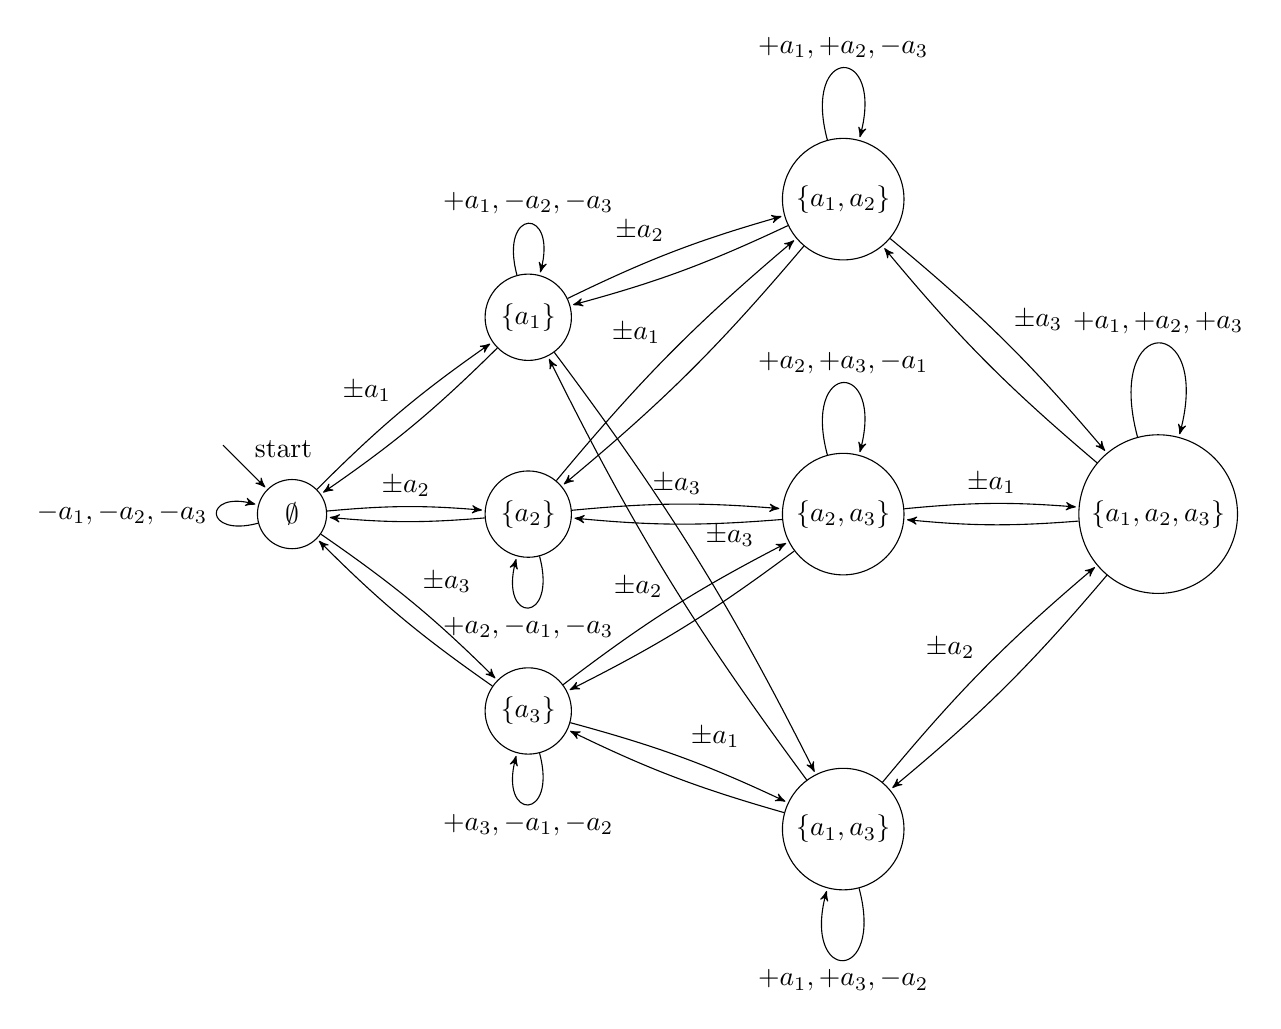
\begin{tikzpicture}[->,>=stealth',shorten >=1pt,auto,node distance=4cm,
	thin, bend angle=5]
	\node[state] (empty) at (0,0) {$\emptyset$};
	\node (hidden) at (-1,1) {};
	\node[state] (a1) at (3,2.5) {$\{a_1\}$};
	\node[state] (a2) at (3, 0) {$\{a_2\}$};
	\node[state] (a3) at (3,-2.5) {$\{a_3\}$};
	\node[state] (a12) at (7, 4) {$\{a_1,a_2\}$};
	\node[state] (a23) at (7,0) {$\{a_2,a_3\}$};
	\node[state] (a13) at (7,-4) {$\{a_1,a_3\}$};
	\node[state] (a123) at (11, 0) {$\{a_1,a_2,a_3\}$};
	
	\path (hidden) edge node {start} (empty);
	
	\path (empty) edge [bend left] node {$\pm a_1$} (a1)
	edge [bend left] node {$\pm a_2$} (a2)
	edge [bend left] node {$\pm a_3$} (a3)
	edge [loop left] node {$-a_1,-a_2,-a_3$} (empty);
	
	\path (a1) edge [loop above] node {$+ a_1, -a_2, -a_3$} (a1)
	edge [bend left] node {$\pm a_2$} (a12)
	edge [bend left] node {$\pm a_3$} (a13)
	edge [bend left]  (empty);
	
	\path (a2) edge [loop below] node {$+a_2, -a_1, -a_3$} (a2)
	edge [bend left] node {$\pm a_1$} (a12)
	edge [bend left] node {$\pm a_3$} (a23)
	edge [bend left] (empty);
	
	\path (a3) edge [loop below] node {$+a_3, -a_1, -a_2$} (a3)
	edge [bend left] node {$\pm a_1$} (a13)
	edge [bend left] node {$\pm a_2$} (a23)
	edge [bend left] (empty);
	
	\path (a12) edge [loop above] node {$+a_1,+a_2, -a_3$} (a12)
	edge [bend left]  (a2)
	edge [bend left]  (a1)
	edge [bend left] node {$\pm a_3$} (a123);
	
	\path (a23) edge [loop above] node {$+a_2,+a_3, -a_1$} (a12)
	edge [bend left]  (a2)
	edge [bend left]  (a3)
	edge [bend left] node {$\pm a_1$} (a123);
	
	\path (a13) edge [loop below] node {$+a_1,+a_3, -a_2$} (a13)
	edge [bend left]  (a1)
	edge [bend left]  (a3)
	edge [bend left] node {$\pm a_2$} (a123);
	
	\path (a123) edge [loop above] node {$+a_1,+a_2,+a_3$} (a13)
	edge [bend left]  (a12)
	edge [bend left]  (a23)
	edge [bend left]  (a13);
	\end{tikzpicture}
	\caption{The result of the add and remove item operations on the bag machine with the set of \texttt{ITEMS} being $\{a_1, a_2, a_3\}$. Each of the labels of the form '$\pm a_i$' refers to both edges connecting the corresponding nodes.}
	\end{figure*}
	\subsection{Discussion of the specification}
	We take the metaphorical bag to be as generic as possible and attempt to interpret the specification in any reasonable way. The details are deliberately left up to interpretation - for example it is not specified whether multiple copies of an item can be included or not, thus making the content of a bag into a set following the Zermelo-Fraenkel definition, or a multiset. Both possibilities will be explored.
	
	An image of a bag of items was chosen due to its simplicity, although we recognize that it is potentially an unhelpful deviation from the most general description of this scenario, which can be achieved solely in set-theoretical terminology. We argue that this scenario is applicable in many circumstances. For example, one may be asked to develop a system that controls the barriers to a private car park. Then the system would maintain a set of registration numbers of the vehicles permitted to park there, which is a subset of all possible registration numbers. Another example is a library system, where \texttt{ITEMS} is the set of books in the library, and \texttt{content} are the books a person has on loan. We may want to impose a limit on the total number of items in the subset - bound by the number of spaces in the car park or the maximum number of books permitted to have on loan at the same time. This variation, although not explicitly required by the specification, was analysed in depth among others listed below.
	
	The aim of this scenario is to explore different ways of expressing sets and operations on them. The two sets we are working on are \texttt{ITEMS}, consisting of all possible items that can be put in the bag, and \texttt{content}, the items contained in the bag at a given point. There are various ways of describing each of these sets. 
	
	We take the relation between them firstly to be that of subset, namely \texttt{content} $\subseteq$ \texttt{ITEMS} or equivalently \texttt{content} $\in \mathbb{P}(\texttt{ITEMS})$. This already shows two different ways of expressing a simple relation like this. Furthermore we may want to impose the limitation that the content of the bag is a finite set, thus arriving at \texttt{content} $\in \texttt{FIN}(\texttt{ITEMS})$ in B notation, where \texttt{FIN}(\texttt{ITEMS}) denotes all finite subsets of the set of \texttt{ITEMS}. 
	
	There are other ways of describing the relation between the \texttt{ITEMS} and the \texttt{content} of the bag. For example latter can be a mapping from a subset of \texttt{ITEMS} to the number of times a given item appears in the bag.
	
	At the level of abstract machines, it is permitted to use set comprehension and other operations and properties of sets, according to the Zermelo-Fraenkel set theory. The B language offers abbreviations of some more common expressions, such as domain or range restrictions. Another thing for us to explore is how using these shorthand expressions rather than writing them out fully affects the proof process.

	\subsection{Variants of the Bag Machine}
	There are various ways of expressing the requirements given in the specification as an abstract machine. The following files are contained in the \emph{Test\_scenarios} archive to be referenced by the reader. We begin by having \texttt{ITEMS} as a deferred set - a set which will be defined at some later point of the development process, and \texttt{content} as simply a subset of \texttt{ITEMS}, then inspect different ways of including the set of \texttt{ITEMS} in the machine, then we focus on the relation between the two sets as expressed in the Invariant clause. We then move onto different ways of expressing the set of \texttt{ITEMS}, for example as an enumerated set or one of a basic type. We finally explore various ways of describing the content of the bag, such as using sequences or relations. The reason for this order of tasks is to begin with the most intuitive implementation of the specification, before discussing less obvious changes to it.
	
	\subsubsection{Bagmch} is the reference machine which we take to be the core of this scenario. It implements exactly the specification without imposing any non-required conditions, such as the limit on the number of items in the bag. At the same time it includes one condition not explicitly mentioned in the specification, namely:
	\begin{lstlisting}
	INVARIANT
		content : FIN(ITEMS)
	\end{lstlisting}

	The specification requires only that $\texttt{content} \subseteq \texttt{ITEMS}$, however in any implementation it is infeasible to have truly infinite sets, thus the software considers them to be erroneous. In the \emph{B Language Reference Manual}\cite{b reference} we find the following definition for the set of natural numbers: ${\texttt{NAT}  = 0 .. \texttt{MAXINT}}$, where \texttt{MAXINT} can be set by the user for a given project, although it is usually understood to be $2^{31}-1$. This definition is not supported by the \emph{B-book}, thus demonstrating a small disparity between the theory of the B-method and its implementation in Atelier B. Nevertheless it is very reasonable for practical purposes.
	
	This machine generates only four proof obligations and all of them are discharged automatically. The first three check that the Invariant is preserved in the Initialisation and by the operations to add and remove items - the only three actions affecting the state of the bag. The last one is as follows:
	
	\begin{lstlisting}
		"Well definedness" 
	=> 
		content: FIN(content)
	\end{lstlisting}
	
	It is concerned with the well-defineness of the operation \texttt{howmany}, which returns the number of items in the bag. The well-defineness proof obligations arise when an expression is used which requires certain conditions to be met in order to be well-defined. In this case, \texttt{card(content)} is well-defined only if \texttt{content} is a finite set. The well-definess conditions for all such expressions can be found in \emph{B Language Reference Manual}\cite{b reference}. The following machine illustrates the proof obligations generated when the well-definess conditions are not met.
	
	This machine is shown in Appendix A for ease of access.
	
	\subsubsection{Bagmch\_unbounded} illustrates the necessity to impose finiteness on the set of items contained in the bag. The sole difference between this and the reference Bag Machine is the statement:
	
	\begin{lstlisting}
	INVARIANT
		content <: ITEMS
	\end{lstlisting}
	This machine generates the same four proof obligations as the reference machine, however the last one remains undischarged by the automated prover and correctly points the user to a problem in the abstract machine.

	\subsubsection{Bagmch\_pre} shows a workaround the well-defineness proof obligation in the previous example, by adding the goal of the proof obligation to the precondition of the operation rather than the Invariant. It results in one fewer proof obligation than the reference \emph{Bagmch}, as putting the goal of the well-defineness proof obligation in the pre-condition of the related operation prevents the proof obligation from being generated.
	
	While it is a way to avoid dealing with a potentially tricky proof obligation, it only postpones the problem, as preconditions will have to be further specified at the later stages of development. Hence, it may be good enough if the aim is simply to formalize a specification, but this solution will have disadvantages if the abstract machine is intended to be refined all the way to the implementation level. 
	
	\subsubsection{Bagmch\_restrictive} uses more restrictive preconditions on the operations to add or remove an item. In the former case, the precondition is now \texttt{aa : ITEMS-content}. In the case of the remove item operation, it is \texttt{aa : content}. Note that by the nature of the behaviour of the operations is unspecified at this stage, when the precondition does not hold - it is something that will be done at the later stages of development. Hence as long as the preconditions hold, these operations will always change the value of the \texttt{content} variable.
		\begin{figure*}
		\centering
		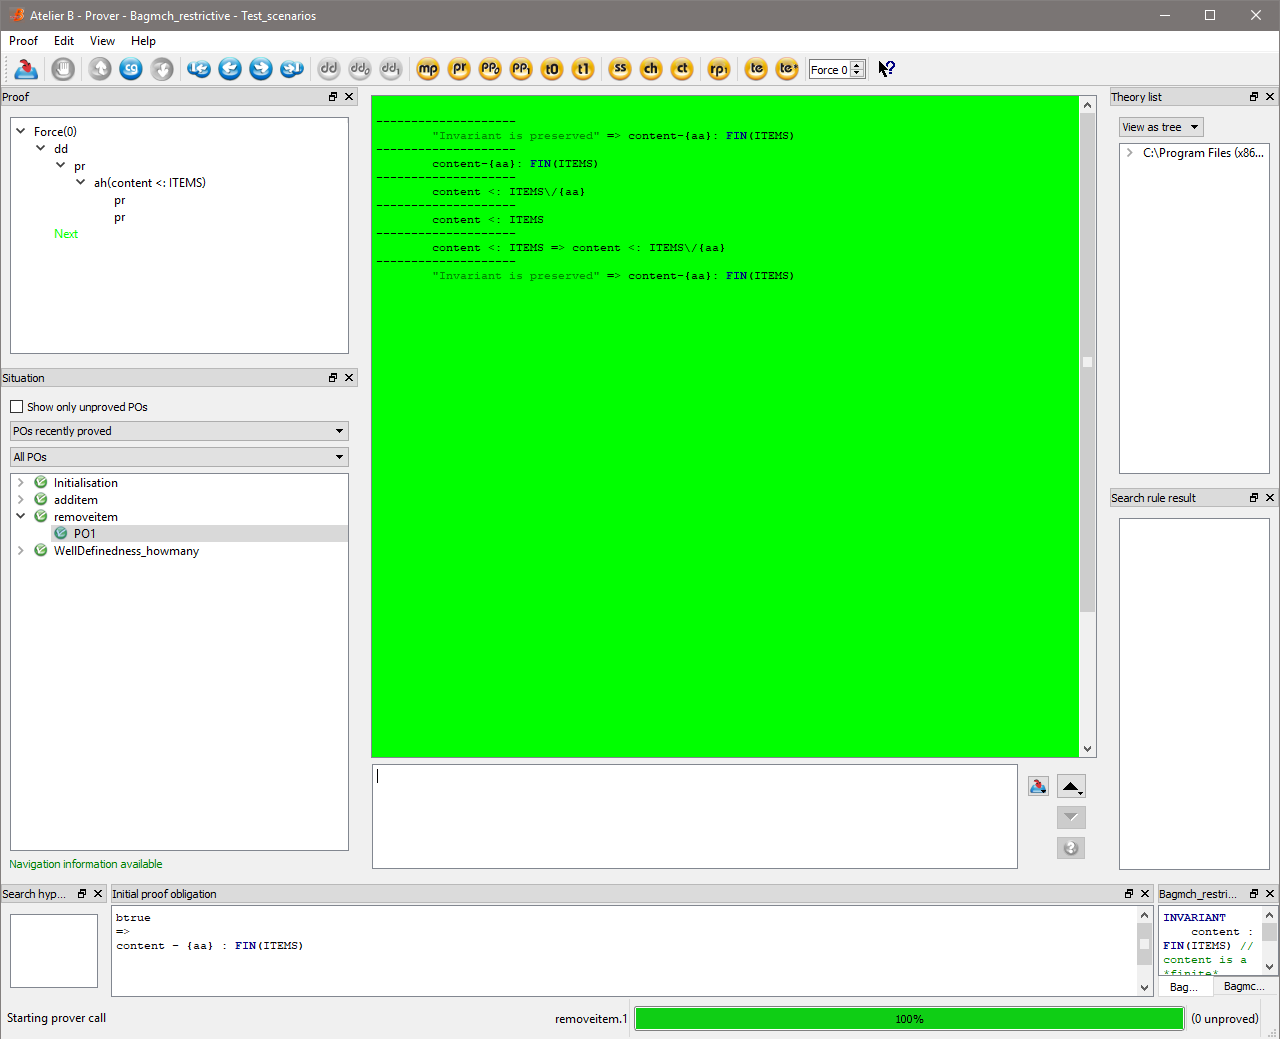
\includegraphics[scale=0.5]{bagmch_restrictive_ip.png}
		\caption{The result of the user pass on the undemonstrated proof obligation in  \emph{Bagmch\_restrictive}.}
		
	\end{figure*}
	This machine results in the same four proof obligations being generated, but now one of them is not discharged automatically. It is the proof obligations regarding the remove item operation, with the goal '\texttt{content-\{aa\}: FIN(ITEMS)}'. Since it is established in the Invariant that \texttt{content} is a subset of \texttt{ITEMS}, the proof obligation is rather trivial. 
	
	There are a couple workarounds to discharge it automatically, however they may not be considered relevant, since they repeat the information already included in the Invariant. Firstly, the condition which is known to be accepted automatically can be added as a conjunct, i.e. the precondition clause of the operation may be turned into '\texttt{aa : content \& aa : ITEMS}'. This addition is redundant, since the Invariant states that \texttt{content} is a subset of \texttt{ITEMS}, but it guides the automatic prover along. This suffices to discharge the proof obligation with the automatic prover, however it also requires the prior knowledge or at least an inclination of what might work.
	
	The second option is to add the clause '\texttt{content <: ITEMS}' to the precondition - we know that it will hold, since the Invariant contains the even more restrictive expression '\texttt{content :  FIN(ITEMS)}'. Adding the third option, the conjunct taken from the Invariant, verbatim, does not result in an automatic demonstration of this proof obligation. This behaviour will be later discussed in \emph{Bagmch\_long\_inv}

	
	We take this opportunity to ease into using the interactive prover. Following the advice from the \emph{Interactive Prover User Manual}, we run the deduction command (\texttt{dd}), and then attempt to get the automated prover to move the proof along further with the \texttt{pr} command. The resultant proof tree is:
	
	\begin{lstlisting}
	--------------------
	"Invariant is preserved" 
=> 
	content-{aa}: FIN(ITEMS) 
	--------------------
	content-{aa}: FIN(ITEMS) 
	--------------------
	content <: ITEMS\/{aa} 
	\end{lstlisting}
	
	The automated prover does not progress further, however this goal is quite trivial, since $\texttt{content} \subseteq \texttt{ITEMS}$ implies that $\texttt{content} \subseteq \texttt{ITEMS} \cup \{\texttt{aa}\}$, and this hypothesis is included indirectly in the Invariant. Thus we can add it with the add hypothesis command: '\texttt{ah(content <: ITEMS)}', and finish the task with the automated prover. 
	
	This suffices to discharge the proof obligation and the above process gets recorded in the \emph{Bagmch\_restrictive.pmm} file, which contains user passes in the interactive prover and component-specific user rules. It can be accessed through the interactive prover and now includes the following as part of the \texttt{User\_Pass} theory:
	
	\begin{lstlisting}
Operation(removeitem) & ff(0) & dd & pr 
& ah(content <: ITEMS) & pr & pr
	\end{lstlisting}
	Where \texttt{ff(0)} denotes automatic proof with force parameter equal to 0 - i.e. with the shortest timeout, the default being 10 seconds, since in a simple scenario like this the prover is not expected to process proof obligations for long. 
	
	Figure 3 shows what performing the user pass looks like in the prover.
	
	\subsubsection{Bagmch\_nondet} is a variation on the \emph{Bagmch} which illustrates how else the specification may be understood. In this machine, the operations to add or remove an item choose the item nondeterministically from the set of \texttt{ITEMS}, rather than accepting a parameter. Nondeterminism is a useful feature at this stage of development, as it helps the user focus on one thing at a time, for example on the action of the operation, rather than the values which are or are not accepted by it.

	The behaviour of this machine is identical to that of the reference machine, with exactly the same four proof obligations being generated and discharged automatically. 
	
	Analogously we can restrict the operation to pick the items from the smaller sets as in the preconditions in \emph{Bagmch\_restrictive}. Note that this conditions are now included not in the \texttt{PRE} section of the operation, but inside the \texttt{ANY} statement. The behaviour is the same as that of \emph{Bagmch\_restrictive}, with the same user pass required to discharge the fourth proof obligation.
	
	\subsubsection{Bagmch\_params} differs from the reference machine in the way the set of \texttt{ITEMS} is included in it. \emph{Bagmch} is given the set of \texttt{ITEMS} as a deferred set, which is required to be explicitly defined at a later stage of the development. Here, it is given as a set-valued parameter, which must be instantiated any time the machine is used.\cite{b-method} However at the stage of abstract machine which is not used by any other machine, it does not make a difference in the prover.
	
	Similar behaviour can be observed later in the machines \emph{Bagmch\_limited} and \emph{Bagmch\_limited\_params}, with a scalar-valued parameter.
	
	\subsubsection{Bagmch\_long\_inv} demonstrates that a provably equivalent way of writing an expression may lead to a different behaviour of the prover. 
	
	There are multiple ways to denote subsets and finite subsets in these two machines. For unbounded subsets \texttt{content} $\subseteq$ \texttt{ITEMS} is equivalent to \texttt{content} $\in$ \texttt{POW(ITEMS)}. We include the latter form in the Invariant of this machine
	
	As we have discovered earlier, we need to limit the content of the bag to only finite subsets of \texttt{ITEMS} in the Invariant clause. A phrasing has been suggested by the well-defineness proof obligation generated by the reference machine. Thus, another way of expressing it to the one seen in the \emph{Bagmch} is:
	
	\begin{lstlisting}
	INVARIANT
	    content : POW(ITEMS) & 
		content : FIN(content) 
	\end{lstlisting}
	
	This time there are six proof obligations generated, all discharged automatically, and they are concerned only with the Invariant being preserved. There is a proof obligation for each clause of the Invariant, one for the Initialisation and one for each of the two operations affecting the content of the bag. 
	
	Firstly, comparing the proof obligation related to the first clause of the Invariant, we see that it is not as simple as the one in \emph{Bagmch\_unbounded}. For example in the Initialisation we see:
	
	\begin{lstlisting}
"Invariant is preserved" &
"Check invariant ((content):(POW(ITEMS)))" 
=>
	{} <: ITEMS 
	\end{lstlisting}

	Where we previously had:
	\begin{lstlisting}
"Invariant is preserved" => {} <: ITEMS 
	\end{lstlisting}
	
	It strongly suggests that the notation $a \subseteq b$ is preferable to $a \in \mathbb{P}(b)$, for any two sets $a$ and $b$. While the result is still the same, the former seems to require less work from the prover, since fewer clauses are generated. Thus especially for large projects may save some computation time. 
	
	Next we compare the proof obligations regarding finiteness of \texttt{content}. The one generated now are of the form:
	
	\begin{lstlisting}
"Invariant is preserved" &
"Check invariant ((content):(POW(ITEMS)))" 
=>
	{} : FIN({}) 
	\end{lstlisting}
	
	We can compare it to the finiteness POs in the reference \emph{Bagmch}:
	
	\begin{lstlisting}
"Invariant is preserved" => {}: FIN(ITEMS)  
	\end{lstlisting}
	
	This change in expression does not appear to make a difference for the proof obligations regarding the Invariant being preserved. However the key distinction between this machine and the reference is that now there is now no proof obligation concerning the well-defineness of the expression \texttt{card(content)}. In this case, by adding the goal of a proof obligation regarding well-defineness, as it was seen before, to the Invariant, we have avoided the proof obligation altogether. A similar behaviour will be observed in later examples.
	
	We conclude that these two ways of expressing the relation '\texttt{content} is a finite subset of \texttt{ITEMS}', while equivalent in theory, will affect the performance and the time taken to complete computations by the prover in different ways. One will result in more proof obligations being generated, however they will be of a simpler nature and discharged automatically, which is faster than discharging even a single proof obligation manually, such as the well-defineness one in the latter case. We recognize that it is something that may be noticeable at large-scale projects, while in a small scenario the overhead will severely affect any measurements of performance, and therefore we have no means of exploring it further in this work, but we highlight it as something users should be aware of.
	
	It is regrettable that the prover not allow us to inspect the proof rules applied when proof obligations are automatically discharged, leaving us with speculations about its inner workings.
	       
	\subsubsection{Bagmch\_finite\_items} is an attempt to impose finiteness earlier on, on the set of \texttt{ITEMS}. We do it by adding the expression '$\texttt{ITEMS} \in \texttt{FIN(ITEMS)}$' to the Properties clause. Otherwise the machine is identical to \emph{Bagmch\_unbounded}. We rely on the fact that any subset of a finite set is necessarily finite. Appendix B contains a proof of this claim.
	
	We see the same four proof obligations as in \emph{Bagmch\_unbounded}, and again the one regarding well-defineness is not discharged automatically. We can of course add the clause '$\texttt{content} \in \texttt{FIN(content)}$' or otherwise explicitly impose the finiteness property on the contents of the bag, but it should not be necessary. The machine is correct, and as the aforementioned proof suggests, it can be verified manually.
	
	Thus we move on to the next stage in our process, as described in the Methodology section. The interactive prover allows users to search rules by the goal, as well as browse the file containing the integrated proof rule base. However none of the rules contains the goal required. No other manipulation in the interactive prover, nor the application of the predicate prover leads to discharging the proof obligation either.
	
	The claim 'a subset of a finite set is finite' can be expressed as a B rule as follows:
		
	\begin{lstlisting}
	THEORY userInFINXY IS
		band(binhyp(b: FIN(b)), 
		binhyp(a <: b))
		=>
		a: FIN(a)
	END
	\end{lstlisting}
	
	The notation means that the conjuncts (AND) of the two hypotheses: 'b is a finite set' and '$a \subseteq b$' implies the goal, that a is a finite set as well.
	
	This rule can be added to the \emph{.pmm} file for this component, so that it is not visible during other proofs, or to the Patch Prover, which contains user-added rules available to all components in a project. Either way it has to be then called explicitly in the interactive prover, with the command to apply rule '\texttt{ar(<theory name>)}', to discharge the obligations with this goal. The project archive contains the \emph{Bagmch\_finite\_items.pmm} file with this rule to illustrate how it works. 
	
	An alternative to including this rule in the PatchProver or the \emph{.pmm} file is to add the goal of the proof obligation to the Invariant, as can be seen in \emph{Bagmch\_long\_inv}. This is a safer alternative, because it will certainly not permit incorrect statements to be accepted by the prover, although it may restrict the number of legal states of the machine. At the same time it leads to more proof obligations and it can be considered the user performing part of the proof manually.
	
	To use this rule in the prover, the user has to make a call to the 'apply rule' command: '\texttt{(ar(userInFINXY))}'. This discharges the proof obligation, and the user pass is saved as follows:
\begin{lstlisting}
Operation(WellDefinedness_howmany) & 
ff(0) & dd & pr & ar(userInFINXY)
	\end{lstlisting}
	
	\subsubsection{Bagmch\_constant\_set} is very similar to the previous machines. This time the superset of \texttt{content} is a set described in the Constants clause, with the following properties:
	
	\begin{lstlisting}
	CONSTANTS
		items
	PROPERTIES
		items : FIN(ITEMS)
	\end{lstlisting}
	Thus we arrive at a sequence: $\texttt{content} \subseteq \texttt{items} \subseteq \texttt{ITEMS}$.
	
	The behaviour of this constant is identical to that of the deferred set of \texttt{ITEMS}, as seen in \emph{Bagmch\_finite\_items}.
	
	\subsubsection{Bagmch\_constant\_set2} is a combination of the previous two machines. The finiteness is imposed on the set of \texttt{ITEMS}, but the sets are related as in \emph{Bagmch\_constant\_set}. This is captured in the Properties clause:
	\begin{lstlisting}
	PROPERTIES
		ITEMS : FIN(ITEMS)
		items <: ITEMS 
	\end{lstlisting}
	The \texttt{howmany} operation generates the well-defineness proof obligation as expected, and it does not get discharged automatically. This time it is really necessary to guide the interactive prover along. The prover does not deal well with the sequence of sets, and the user is required to take the interactive prover through it step by step. First it is necessary add a hypothesis that \texttt{items} is a finite set - using the command \texttt{ar(items : FIN(items))}, then apply the rule which was discussed earlier, twice. 
	
	The whole process, including the user input, is recorded in the user pass file and the part regarding the troublesome proof obligation looks as follows:
	
	\begin{lstlisting}
Operation(WellDefinedness_howmany) & 
ff(0) & pr & ah(items : FIN(items)) &
ar(userInFINXY) & pr & ar(userInFINXY)
	\end{lstlisting}
	Where \texttt{ff(0)} denotes automatic proof with force parameter equal to 0, which was done automatically already, the command \texttt{pr} is simply a call to the automatic prover, and \texttt{ar(<theory name>)} is applying the user-created rule as before. Adding a hypothesis means that, if the goal is $G$, the current hypotheses are $h_1, ..., h_n$, and the new one $P$, then the prover will first attempt to demonstrate $P$ under the hypotheses $h_1, ..., h_n$, and then prove $G$ under the hypotheses $h_1, ...,h_n, P$.\cite{PO reference}  Thus the additional hypothesis has to be demonstrated first, which is the reason for applying the added rule twice. 
	
	This is a clear inconvenience when a proof requires a longer sequence of sets to have a certain property proven one by one. Fortunately, user passes as the one listed above can be added to the component's \emph{.pmm} file and called to perform the sequence of commands with a single input from the user, as described in Chapter 5 of the \emph{Proof Obligations Reference Manual}.
	
	
	\subsubsection{Bagmch\_limited} imposes a limit on the number of items that can be included in the bag at once. We define this limit as \texttt{max\_elem} in the \texttt{CONSTANTS} clause of the static part of the machine and give its type in the \texttt{PROPERTIES} clause:
	
	\begin{lstlisting}
	CONSTANTS
		max_elem
	PROPERTIES
		max_elem : NAT
	\end{lstlisting}
	
	Here, we explicitly restrict \texttt{max\_elem} to be non-negative. Changing this expression to '$\texttt{max\_elem} \in \mathbb{Z}$' results in an unprovable proof obligation in the Initialisation, the goal of which is $card(\{\}) \leq \texttt{max\_elem}$ for all possible values of \texttt{max\_elem}. It clearly does not hold for negative values of the constant, hence it is limited to natural numbers.
	
	Furthermore, there is no difference between defining just the type of \texttt{max\_elem} or its value, forgoing the type declaration, i.e. having only the clause '\texttt{max\_elem} $= x$' for some chosen $x \in \mathbb{N}$ in the Properties clause. The type of it is defined implicitly and it does not affect the proof process.

	This restriction impacts the \texttt{additem} operation, as we now need to check that adding an item to the bag will not exceed the limit. It can be done in the preconditions section of the operation, as is shown in the example included in the archive, or in an if-else statement. We found these ways to be equivalent for our purposes, as they do not generate different proof obligations. It is worth noting that they will impact the refinement stages of the development. We have elected to stick to the former, since it is less restricting for potential refinement.
	
	There are nine proof obligations generated. The initialisation and each of the operations to add and remove items results in two: one being a type check, the other making sure that the cardinality of \texttt{content} does not exceed \texttt{max\_elem}. The last three proof obligations are concerned with the well-definess of the expression \texttt{card(content)} in the invariant and the operation \texttt{additem} and \texttt{howmany}, that is anywhere where the expression appears.
	
	If the expression $\texttt{content} \in \texttt{FIN(ITEMS)}$ is replaced with $\texttt{content} \subseteq \texttt{ITEMS} \wedge \texttt{content} \in \texttt{FIN(content)}$ there are again nine proof obligations. However this time there are three proof obligations for each of the Initialisation and the adding and removing operations - one proof obligation for each clause of the Invariant. At the same time the well-defineness proof obligations are not generated. This is in line with the observations regarding \emph{Bagmch\_long\_inv}.

	\subsubsection{Bagmch\_limited\_params} differs from the previous version by passing \texttt{max\_elem} as a scalar-valued parameter instead. The software requires defining at least the type of \texttt{max\_elem} in the Constraints clause, while the Constants and Properties clauses can now be removed. As in the case of \emph{Bagmch\_params} with a set-valued parameter, it does not affect the proof process.
	
	\subsubsection{Bagmch\_wrong\_order} is of particular interest, as it highlights a discrepancy between the theory of the B-method and its implementation in Atelier B. The Invariant clause contains a series of conjuncts which by the rules of logic are commutative. However they are not such in the software.
	
	Firstly, recall that in the \emph{Bagmch\_long\_inv}, the Invariant was as follows:
	
	\begin{lstlisting}
	INVARIANT
		content <: ITEMS &
		content : FIN(content)
	\end{lstlisting}
	
	Switching these two statements around results in an error message generated as static analysis is taking place, demanding that the type of \texttt{content} is defined before applying the built-in operator \texttt{FIN} to it. The software does not allow the user to proceed with the proof as long as such errors exist.
	
	With the addition of the limit on the number of items in the bag, this problem becomes much less obvious. For example, if the Invariant is formulated like this:
	
	\begin{lstlisting}
	INVARIANT
		content <: ITEMS &
		card(content) <= max_elem & 
		content : FIN(content)
	\end{lstlisting}
	
	The static analysis does not give any errors, however an additional proof obligation is generated, on top of the nine we get in the alteration to the \emph{Bagmch\_limited} mentioned above. The proof obligation is:
	
	\begin{lstlisting}
    	content <: ITEMS &
		"Well definedness" 
	=>
		content: FIN(content) 
	\end{lstlisting}
	
	It does not get discharged by any means available to the user within the interactive prover.	
	
	Based on these observations we reach the conclusion that the conjuncts in the Invariant are applied sequentially, in the order in which they are written. It is very much like the Assertion clause, which is defined to be checked sequentially in the B method. It is also understandable from the implementation point of view, since checking all permutations of the conjuncts would be computationally hard.
	
	\subsubsection{Bagmch\_redundant...} are five machines with redundant clauses in the Invariant, written in a different order or in a slightly different manner, but essentially nigh identical. Note that it is a very bad practice to do something like this intentionally, however as this work is aimed at people beginning their work with the B method, it is expected that a similar mistake, albeit a less obvious one, can happen.
	
	They borrow the concept of imposing the maximum number of items that can fit in the bag from the previous machines. This time we add redundant clauses in the Invariant to explore the relation between their number and the number of proof obligations generated, as well as observe if there is any evidence of optimisation in the prover.
	
	We begin with \emph{Bagmch\_redundant}. Just like in \emph{Bagmch\_limited} it has a constant \texttt{max\_elem} which is then described in the Properties clause as \texttt{max\_elem : NAT}.
	
	The Invariant now looks as follows:
	\begin{lstlisting}
INVARIANT
	content : POW(ITEMS) & 
	content : FIN(content) &
	card(content) <= max_elem + 4 &
	card(content) <= max_elem + 3 &
	card(content) <= max_elem + 2 &
	card(content) <= max_elem + 1 &
	card(content) <= max_elem
	\end{lstlisting}
	Firstly note that the third, fourth, fifth, and sixth clauses are redundant - it is sufficient that the last clause holds for these four to also hold. At the same time it is a very simple way of creating an arbitrary number of Invariant clauses. Also, observe that we have used the more explicit way of describing the type and finiteness of \texttt{content} - as a separate clause for each of those requirement, as seen in \emph{Bagmch\_long\_inv}. This way we avoid the well-defineness proof obligations.
	
	There are 21 proof obligations generated in this case - 7 for each of the two operations affecting \texttt{content} and 7 more for the Initialisation. The Initialisation and the operation to add an item have all their proof obligations discharged automatically. Surprisingly, out of the five cardinality-related proof obligations for the operation to remove an item, only the simplest on, namely the one regarding the clause \texttt{card(content) <= max\_elem}, gets discharged automatically. The other ones require user input in the interactive prover. 
	
	They can still be discharged without creating additional rules. For each one of them, the same steps work, since their structure is identical. Each one has two goals - one for the case when the item the operation is removing is an element of \texttt{content}, the other when it is not. Their initial goal is of the same form as the simple proof obligation:
	\begin{lstlisting}
card(content-{aa})<=max_elem+1 
	\end{lstlisting}
	If we run the 'prove' command (denoted by 'pr' in the prover), the goal is rewritten into:
	\begin{lstlisting}
0<=1+max_elem-card(content-{aa}) 
	\end{lstlisting}
	
	We notice that the simplest proof obligation was discharged, so we add a hypothesis consisting of it rewritten in the way appearing in the goal. It is done with the command:
	\begin{lstlisting}
ah(0<=max_elem-card(content-{aa}))
	\end{lstlisting}
	Where 'ah' stands for the 'add hypothesis' command. We then prove this additional hypothesis with 'prove' and the goal turns into:
	\begin{lstlisting}
0<=max_elem-card(content-{aa}) 
=> 0<=1+max_elem-card(content-{aa}) 
	\end{lstlisting}
	Running 'prove' again satisfies this goal and moves onto the next one: 
	\begin{lstlisting}
not(aa: content) 
=> 0<=1+max_elem-card(content)
	\end{lstlisting}
	This one is satisfied with just the 'prove' command. Thus the User Pass for the operation 'removeitem' is recorded as follows:
	\begin{lstlisting}
Operation(removeitem) & ff(0) & pr & 
ah(0<=max_elem-card(content-{aa})) & 
pr & pr & pr
	\end{lstlisting}
	We have found a way of discharging these proof obligations, by comparing the goal to one which the prover has successfully dealt with before. We have essentially given the prover a simpler hypothesis, stripped of the additional scalar constants.
	
	We do not have an explanation for why these proof obligations have been problematic. The prover has not timed out while processing them, and indeed attempting to discharge them with a greater force parameter does not change the outcome.
	
	\emph{Bagmch\_redundant2} uses a Definition clause as follows:
	\begin{lstlisting}
DEFINITIONS
	max_elem == 3
	\end{lstlisting}
	It is equivalent to defining \texttt{max\_elem} as a constant in the Constants clause and giving it a value in the Properties clause. This method is advised by the \emph{Interactive Prover User Manual}\cite{Prover guide}, which claims that it prevents the prover from performing avoidable replacements. \emph{Bagmch\_redundant3} differs by replacing the expressions '\texttt{max\_elem + n}' by concrete natural numbers. In both cases all of the proof obligations are discharged automatically.
	
	Given the previous findings about the conjuncts in the Invariant not being commutative, we have also explored ordering the clauses from the most to the least restrictive - i.e. reversing the order of the conjuncts from the Invariant shown above. We found that it did not change the outcome in this case. In \emph{Bagmch\_redundant\_reverse} \texttt{max\_elem : NAT} is used just like in \emph{Bagmch\_redundant} and the same proof obligations are generated and not discharged. In \emph{Bagmch\_redundant\_reverse2} we use numerical values instead of a constant in each conjunct, and all proof obligations are observed to discharge automatically.
	
	Finally we have tried including the same conjunct twice in the Invariant, and only then we have noticed that the redundancy is acted upon by the software - the prover does not list the same conjunct twice. 
	
	We move on to discuss the number of proof obligation generated in relation to the number of clauses in the Invariant. Recall that the machine has two operations which change the \texttt{content} variable. Each one of them and the Initialisation generates one proof obligation for each clause in the Invariant. With the Invariant as given above, it comes to three sets of seven proof obligations. 
	
	Adding clauses following the pattern '\texttt{card(content) <= max\_elem + n}' and checking the number of generated proof obligations gives rise toto the following observation about the number of proof obligations concerned with the preservation of the invariant. The number of proof obligations is equal to the number of operations affecting the state of the machine multiplied by the number of conjuncts in the Invariant. We will inspect the proof obligations generated for the Initialisation later.	
	
	Note that at this point all the clauses are related to the single variable affected by the operations. We will see if having clauses concerning other variables, unaffected by these operations, changes the pattern in \emph{Bagmch\_2sets}.
	
	\subsubsection{Bagmch\_2sets} allows us to further investigate the relation between the number of proof obligations and clauses in the Invariant. This machine maintains two subsets of \texttt{ITEMS}, called \texttt{content1} and \texttt{content2}. They act exactly like the \texttt{content} set did in the previous machine. We thus have two conjuncts involving each of the variables in turn, and for the sake of observing all factors, we add an additional (redundant) conjunct involving both variables, so the Invariant now becomes:
	
	\begin{lstlisting}
	INVARIANT
		content1 <: ITEMS &
		content1 : FIN(content1) &
		content2 <:ITEMS &
		content2 : FIN(content2) &
		content1 \/ content2 <:ITEMS
	\end{lstlisting}
	The longer, more explicit Invariant was chosen to avoid having to deal with proof obligations related to well-defineness, and focus on those concerning the preservation of the Invariant.
	
	The two sets are initialised to the same value, the empty set. That is, the Initialisation clause contains only the parallel assignment: 
	\begin{lstlisting}
	INITIALISATION
		content1 := {} || content2 := {}
	\end{lstlisting}
	
	Each one of the sets has their own copy of the familiar operations to add and remove items. Additionally there is an operation changing both variables simultaneously, to compare the number of proof obligations it generates next to the former ones. The operation is as follows:
	
	\begin{lstlisting}
	additemboth(aa) =
	PRE
		aa : ITEMS
	THEN
		content1 := content1 \/ {aa} ||
		content2 := content2 \/ {aa}
	END;
	\end{lstlisting}
	
	As can be expected, each of the operations generate a proof obligation for each conjunct of the Invariant which involves a variable affected by the operation. That is, the operation \texttt{additem1}, which adds an element to \texttt{content1} gives three proof obligations - for the first, third and fifth conjuncts, but not the ones involving \texttt{content2}. The operation adding an item to both sets results in five proof obligations, one for each of the conjuncts.
	
	The proof obligations arising from the Initialisation are much more puzzling. There is only three of them, with the following goals:
	\begin{itemize}
		\item \verb|{} <: ITEMS |
		\item \verb|{}: FIN({}) |
		\item \verb|{}\/{} <: ITEMS|
	\end{itemize}
	The proof obligations did not get duplicated for each of the two sets, which was not in line with our expectations. In fact neither of those three proof obligations refers directly to one variable or the other. 
	
	We will explore this further in the next machine:
	
	\subsubsection{Bagmch\_2sets\_1elem} differs from the previous machine by the Initialisation clause. Instead of starting with an empty set for each of the two variables, the variables are initialised to the same value - a singleton set, containing a nondeterministically chosen element. 
	
	It turns out to be still simple enough for the prover to generate only three proof obligations for the Initialisation preserving the Invariant, as seen in the previous example.
	
	It is not the case in the following variant:
	
	\subsubsection{Bagmch\_2sets\_2elem} nondeterministically picks two elements, \texttt{xx} and \texttt{yy} of the set of \texttt{ITEMS}, and in the Initialisation it assigns the singleton set \texttt{\{xx\}} to \texttt{content1} and \texttt{\{yy\}} to \texttt{content2}. Note that the two chosen items may or may not be the same one. 
	
	Now we observe five proof obligations generated for the Initialisation clause preserving the Invariant - one for each conjunct in the Invariant, since the initial values for the two variables may now differ.
	
	We conclude that the automated prover optimizes enough to not repeat the exactly same chunk of work twice, for example when two conjuncts of the Invariant are identical or when two assignments would generate exactly the same goals in proof obligations. However its ability to optimise does not go as far as to notice for example that the behaviour of a singleton subset of \texttt{ITEMS} will be the same in our examples, regardless of its actual value. That is not unexpected, and the software should be commended for not over-optimising, but still having some basic optimisation built in.
	
	\subsubsection{Bagmch\_setops} briefly explores if operations taking finite subsets of \texttt{ITEMS} as parameters instead of a single element of that set, make any difference to the proof process. This change does not appear to have any impact on the proof process, as compared to the reference \emph{Bagmch}.
	
	\subsubsection{Bagmch\_enum} strays from the set of \texttt{ITEMS} being deferred, as can be seen in all previous machines. Instead, it is defined explicitly as an enumerated set with three elements, namely \texttt{ITEMS = \{FOO, BAR, BAZZ\}}. It is a copy of the reference \emph{Bagmch}, the only difference being the definition of the set of \texttt{ITEMS}. The operations all remain the same as before.
	
	The reason for this change is to explore the behaviour of enumerated sets as they are implemented in the Atelier B. The user manuals do not elaborate on the topic, noting only that "Every enumerated set is dfined as the set comprising all of its elements, and the
	elements are distinct two by two"\cite{PO reference}.
	
	This time we see eight proof obligations, and only two of them are discharged automatically. They are the single proof obligation generated for the Invariant, with the goal \texttt{\{\}: FIN(ITEMS)}, and the one concerned with the well-defineness of the expression involving cardinality in the operation 'howmany'. Its goal is: \texttt{content: FIN(content)}.
	
	The other six come from the operations. The three operations that do not affect the value of the variable \texttt{content} result in four proof obligations - one for each of 'getcontent' and 'howmany' operations, and two for 'isin', the latter caused by the if-else statement. All of those four proof obligations have the goal '\texttt{content: FIN(ITEMS)}', which is the exact expression present in the Invariant, which defines the type of the variable \texttt{content}. The operations to add or remove item result in proof obligations with goals '\verb|content\/{aa}: FIN(ITEMS)|' and '\verb|content-{aa}: FIN(ITEMS)|' respectively. 
	
	Tackling any of those proof obligations with the prover provides significant insight into the internal implementation of the enumerated set. The prover generates the following subgoals:
	
	\begin{itemize}
		\item \verb|dom(content): FIN(INTEGER)|
		\item \verb|1<=min(dom(content))|
		\item \verb|max(dom(content))<=3|
		\item \verb|ran(content)<:{ITEMS.enum}|
	\end{itemize}
	Thus the goals to confirm the type of a variable which we know to be a subset of an enumerates set given earlier, show that the enumerated set is realised as a relation from a finite subset of the natural numbers to '\texttt{ITEMS.enum}', which we assume to mean the elements we specified as members of the enumerated set's definition. More specifically, it is a bijection from the set $\{1,2,3\}$ to \texttt{ITEMS.enum} $= \{FOO, BAR, BAZZ\}$.
	
	Our previous attempts to reduce the number of undemonstrated proof obligations suggest adding the goal of the proof obligation to the Invariant, in order to specify the properties of the machine further, in a way more susceptible to the automatic proof. However the initial goal, namely '\texttt{content: FIN(ITEMS)}' is already present in the Invariant. 
	
	An attempt to add the four subgoals listed lead to another observation: the expression '\texttt{ITEMS.enum}' is unrecognized and fails at the stage of static analysis.
	
	A certain way to remove these proof obligations from the list of the undischarged ones is to add their goals as a precondition in each operation. We generally do not advise jumping to this solution easily, but seeing as the goals of the proof obligations are correct due to the type definition of \texttt{content}, and that the prover appears to be stumbling over something that in the reference machine was trivially demonstrated, we opt for it. We did not find an explanation for this frustrating behaviour of the software.
	
	Thus, we add '\texttt{content: FIN(ITEMS)}' as a precondition to each operation, since we are interested only in the states of the machine in which this expression is true. Then we re-generate the proof obligations and run the automated prover again. The four proof obligations related to the operations not affecting the value of the variable \texttt{content} disappear entirely. The remaining four are analogous to the ones in the reference \emph{Bagmch} and are discharged by the automated prover.
	
	It is a crude workaround, and one might ask what benefits it gives. Removing proof obligations from the list of the undischarged ones allows the user to focus on other ones, and not be distracted by ones which were analysed and deemed to hold earlier. In fact, the use of preconditions in general is justified by wanting to separate concerns and focus on one thing at a time. Thus this method may be readily applied by users who want to concentrate on more meaningful proof obligations, and is a valid tactic in their situation.
	
	\subsubsection{Bagmch\_relation} explores the possibilities given by the in-built notation and operations on relations and functions in the B language. This time the bag can contain multiple copies of an item. The content of the bag is realised as a partial function from \texttt{ITEMS} to positive integers. Recall that while in set theory functions are realised as sets of ordered pairs, which in this case means subset of $\texttt{ITEMS} \times \texttt{NAT1}$, in the B language they are sets of maplets, each one expressed as '\texttt{aa|->nn}' for some $\texttt{aa} \in \texttt{ITEMS}$ and some $\texttt{nn} \in \texttt{NAT1}$.
	
	The Invariant now looks as follows:
	\begin{lstlisting}
INVARIANT
	content : ITEMS+->NAT1 &
	dom(content) : FIN(ITEMS)
	\end{lstlisting}

	An item is listed in this function only if there is at least one present in the bag. As a result the add and remove item operations have to be split into cases. When adding an item, we can either increase the count if it is already in the bag, or we need to add it to the domain of \texttt{content}. Hence now the operation turns into:
	\begin{lstlisting}
additem(aa) =
PRE
	aa : ITEMS
THEN
	IF 
		aa : dom(content) 
	THEN
		content := content 
			<+ {aa|->content(aa)+1}
	ELSE
		content := content\/{aa|->1}
	END
END;
	\end{lstlisting}
	One can observe the syntax for maplets mentioned earlier, for functional override, denoted \texttt{<+}, and finally that \texttt{content} is still essentially a set, although its elements are now of a different form.
	
	Similarly the operation to remove an item is split into multiple cases. If there is more than one copy of the item in the bag, we decrease the count. If there is precisely one present, we remove the maplet '\texttt{aa|->1}' from the \texttt{content}. Finally, if there is none, the operation does nothing.
	
	Another operation which gets severely affected by this change to the definition of \texttt{content} is the operation returning the total number of items in the bag. At the abstract machine level, it is possible to use summation over a set. It is expressed as \verb=SIGMA(xx).(xx:dom(content)|content(xx))=. 
	
	Note that we cannot simply add all elements in the range of \texttt{content}, because if there are multiple elements appearing in the same quantity, their number will be added only once. That is, if \texttt{content = \{aa|->1, bb|->1\}}, then the range of this function is \texttt{ran(content) = \{1\}}, and summing over it will not give the correct result.
	
	This machine has 13 proof obligations generated, and only one of them is not discharged automatically. This came as a pleasant surprise, and indicates that the structures used are still relatively simple, for example in comparison to the enumerated set.
	
	The problematic proof obligation in fact points to an oversight in the initial abstract machine. Its goal is initially '\texttt{content<+\{aa|->content(aa)+1\}: ITEMS +-> NAT}' and the reason behind it may not be obvious at first, but running the automated prover on it narrows it down to: '\texttt{content(aa)<=2147483646}', the number being the value of the in-built \texttt{MAXINT} constant. Thus the prover is asking the user to make sure that the maximum implemented integer is not exceeded by adding an item.
	
	Hence the behaviour of the operation to add an item has to be restricted in the case when the count of an item in the bag is increased. Adding simply '\texttt{content(aa) < MAXINT}' is not sufficient, since it assumes that \texttt{aa} is in the domain of \texttt{content}, and leads to further difficulties. On the other adding a precondition just to one branch of an if-else statement is impossible. Hence we opt for writing the preconditions of this operation as:
	\begin{lstlisting}
aa: ITEMS &
(aa: dom(content) => content(aa) < MAXINT)
	\end{lstlisting}
	Thus the additional condition applies only in the relevant branch.
	
	This machination results in an additional proof obligation generated, dealing with the well-definess of the preconditions to this operation. It is understandable, since the expression \texttt{content(aa)} is meaningful only if \texttt{aa} is in the domain of the function. 
	
	All of the 14 proof obligations which were generated this time, get demonstrated by the automated prover, without any input from the user.
	
	We further inspect the proof obligations generated for the operation involving the summation. There are two of them, and both are concerned with well-defineness conditions. The lack of proof obligations regarding the preservation of the Invariant is not unexpected, since this operation does not change the state of the machine. The first proof obligation checks that the summation is carried over a finite set. 
	
	The second contains a goal similar to those seen in the other well-defineness proof obligations for this machine, namely '\texttt{content: dom(content) +-> ran(content)}. Although this time it involves set comprehension, that is '\texttt{\{~xx | xx: dom(content)\}}', the meaning is the same. It appears to be a simple type check, to ensure that the structure is understood correctly.
	
	This machine gives an idea of what to expect when dealing with functions, although it is very simplistic and not problematic at all. We hope that even this insight will be useful in working on the second set of machines.
	
	\subsection{Summary}
\begin{figure*}
	\centering
	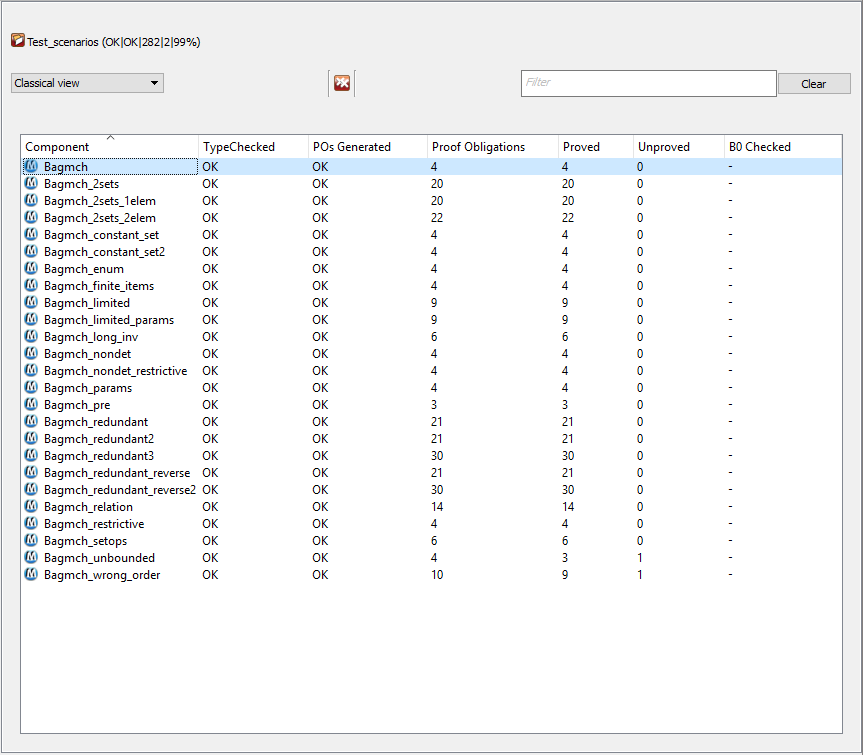
\includegraphics[scale=0.8]{bagmchs.png}
	\caption{Machines which arose from the Bag scenario, as presented in the software}
\end{figure*}
	
\begin{table}[h]
	\centering
\begin{tabular}{@{}rlrr@{}}
	\toprule
	\multicolumn{1}{l}{Section} & Machine                     & \multicolumn{1}{l}{\begin{tabular}[c]{@{}l@{}}Number \\ of POs\end{tabular}} & \multicolumn{1}{l}{\begin{tabular}[c]{@{}l@{}}POs requiring\\ user action\end{tabular}} \\ \midrule
	1                           & Bagmch                      & 4                                                                            & 0                                                                                       \\
	3                           & Bagmch\_pre                 & 3                                                                            & 0                                                                                       \\
	4                           & Bagmch\_restrictive         & 4                                                                            & 1                                                                                       \\
	5                           & Bagmch\_nondet              & 4                                                                            & 0                                                                                       \\
	6                           & Bagmch\_nondet\_restrictive & 4                                                                            & 1                                                                                       \\
	6                           & Bagmch\_params              & 4                                                                            & 0                                                                                       \\
	7                           & Bagmch\_long inv            & 6                                                                            & 0                                                                                       \\
	8                           & Bagmch\_finite items        & 4                                                                            & 1                                                                                       \\
	9                           & Bagmch\_constant set        & 4                                                                            & 1                                                                                       \\
	10                          & Bagmch\_constant set2       & 4                                                                            & 1                                                                                       \\
	11                          & Bagmch\_limited             & 9                                                                            & 0                                                                                       \\
	12                          & Bagmch\_limited\_params     & 9                                                                            & 0                                                                                       \\
	14                          & Bagmch\_redundant           & 21                                                                           & 4                                                                                       \\
	14                          & Bagmch\_redundant2          & 21                                                                           & 0                                                                                       \\
	14                          & Bagmch\_redundant3          & 30                                                                           & 0                                                                                       \\
	14                          & Bagmch\_redundant\_reverse  & 21                                                                           & 4                                                                                       \\
	14                          & Bagmch\_redundant\_reverse2 & 30                                                                           & 0                                                                                       \\
	15                          & Bagmch\_2sets               & 20                                                                           & 0                                                                                       \\
	16                          & Bagmch\_2sets\_1elem        & 20                                                                           & 0                                                                                       \\
	17                          & Bagmch\_2sets\_2elem        & 22                                                                           & 0                                                                                       \\
	18                          & Bagmch\_setops              & 6                                                                            & 0                                                                                       \\
	19                          & Bagmch\_enum                & 8                                                                            & 6                                                                                       \\
	20                          & Bagmch\_relation            & 13                                                                           & 1                                                                                       \\ \bottomrule
\end{tabular}
			
	\caption{List of machines which arose from the Bagmch scenario}
\end{table}
	The machines listed in Table 1 have been included in the attached archive containing the source code and user passes (where relevant). They are listed here for comparison, together with the number of proof obligations generated in the initial version of the machines, before the proof obligations were inspected in the interactive prover and before any changes were done to the code in order to decrease their numbers. Although in all examples we have managed to demonstrate all of them, in Table 1, we note which ones required the use of the interactive prover due to not all proof obligations being discharged automatically.
	
	Two machines were omitted from this list, because they were deliberately left with undischarged proof obligations which point to errors. They are listed in Table 2.
	
	\begin{table}[h]
		\centering
\begin{tabular}{@{}rlrr@{}}
	\toprule
	\multicolumn{1}{l}{Section} & Machine                     & \multicolumn{1}{l}{\begin{tabular}[c]{@{}l@{}}Number \\ of POs\end{tabular}} & \multicolumn{1}{l}{\begin{tabular}[c]{@{}l@{}}POs requiring\\ user action\end{tabular}} \\ \midrule
	2 & Bagmch\_unbounded & 4 & 1  \\
	13 & Bagmch\_wrong\_order & 10 & 1 \\
	\bottomrule
\end{tabular}
		
		\caption{List of machines which contain deliberate, illustrative errors}
	\end{table}

	Figure 4 shows the machines listed above as they would appear in the software.

	\section{Queue, stack, and lists}
	\subsection{Overview and motivation}
	There are many data structures, which cannot be forced into the Bag machine scenario, and trying to do so would be overly contrived and lack clarity. We also stray from the idea of using an abstraction like the Bag, in order to make the reasoning simpler. Instead, we present a collection of machines which do not conform to a specific scenario, but instead focus on typical data structures in computer science in general.
	
	The particular data structures we have translated to B language are:
	\begin{itemize}
		\item queue
		\item stack
		\item linked list
		\item doubly linked list
		\item tree
		\item binary tree
	\end{itemize}
	
	These machines will make use of the functions and sequences as built into the B language, and will deliberately have more intricate relations between variables, and more complicated operations.
	
	Since they deal with data structures which we have not explored yet, we decided to use this opportunity to test how well our method of reducing the number of undischarged proof obligations works without prior knowledge and practice with the expressions involved. 
	
	To this end we keep two copies of each of the machines listed above. The files marked with \emph{\_initial} show what the machines started as and how they changed thanks to the suggestions given by the interactive prover.
	
	\subsection{Data structures machines}
	\subsubsection{Queuemch\_stack} 
	
	Stacks and queues can both be implemented using a sequence, and differ only by the operations performed on it - the signature ones being \textit{push} and \textit{pop} for stack and then \textit{enqueue} and \textit{dequeue} for queue. Thus to avoid unnecessary repetition, these two data structures are implemented in a single machine. The machine contains a single variable called \texttt{list}, the type of which is a sequence of \texttt{ITEMS}. Then the four operations listed above are performed on it.
	
	A sequence in B language is realised as a function from some set of consecutive integers, with the least one being 1, if the subset is not empty, to a subset of some elements of a given type. In this case, a sequence is therefore a function $f:\{1,2,...,n\} \rightarrow \texttt{ITEMS}$, for some $n \in \mathbb{N}$.

	\emph{Queuemch\_stack\_initial} shows the first attempt at formalising the data structure, before the interactive prover was used and any alterations were made to the code. 13 proof obligations are generated, and only seven of them are discharged automatically.
	
	We first observe the six the undischarged proof obligations are of the well-defineness variety. The goal of each of them is '\texttt{list: seq(ran(list))}'. It asks the user to demonstrate that the variable is a sequence of the elements it contains. Since it is still in line with the desired functionality of the machine, this expression is therefore added as another conjunct in the Invariant, which makes the number of the undischarged proof obligations go down to 2, with the new total being 12. This time only two well-definess proof obligations are generated and get demonstrated by the automated prover. 
	
	Each of the four operations now has two proof obligations generated, instead of one, and the Initialisation gives rise two another two. In each pair is one proof obligation for each conjunct in the Invariant, confirming the pattern observed in the previous section.
	
	The two remaining proof obligations are for the \textit{push} and \textit{enqueue} operations, and they have the goal: '\texttt{list<-aa: seq(ran(list<-aa))}'. Running the automated prover on it gives the subgoal: '\verb|list: seq({aa}\/ran(list))|'. Since sequences are not necessarily surjective, this statement can be easily seen to be correct, as $ran(\texttt{list}) \subseteq \{\texttt{aa}\} \cup ran(\texttt{list})$, and so $\texttt{list} \in seq(\{\texttt{aa}\} \cup ran(\texttt{list}))$.
	
	None of the hypothesis we thought of adding made any difference. Before we resort to adding user rules, we can try the predicate prover. The predicate prover on its own is not sufficient, but running the predicate prover with first level hypothesis - since the hypothesis is needed to demonstrate the goal - succeeds, and the proof obligation is demonstrated.
	
	The user pass now contains the following record:
	\begin{lstlisting}
Operation(push) & ff(0) & dd & pr & 
pp(rp.1) & pr;
Operation(enqueue) & ff(0) & dd & 
pr & pp(rp.1) & pr
	\end{lstlisting}
	
	And all 12 proof obligations are discharged.
	
	\subsubsection{Queuemch\_linked}
	
	This is an implementation of a linked list, where the content of the list is stored in a B language's sequence, and there is an additional function called \texttt{next} to maintain pointers. To disambiguate it and to add another layer of complexity, we will consider an injective linked list, where each element can appear only once.
	
	We use a dummy element, which we call \texttt{anchor} to indicate the beginning of the list. It will point to the first element of the list, and the last element will point to it - thus making the \texttt{next} function a bijection.
	
	The operations to remove an item - whether by the item or by its position in the list - are a little more tricky. We cannot simply remove a maplet related to the element, as the resultant mapping will not be a sequence, since the integers in the domain will not be consecutive.
	
	The initial version of this machine can be found in the file \emph{Queuemch\_linked\_initial} and generates 32 proof obligations, 17 of which are not discharged.
	
	We begin by looking at the well-defineness proof obligations. We notice that two have the goal '\texttt{content: seq(ran(content))}' which was seen in the previous machine. Adding it to the Invariant however does not gain us much. There are now 34 proof obligations generated, and still 17 which are not demonstrated automatically.
	
	Most of the remaining well-defineness-related proof obligations can be discharged with the use of predicate prover. Afterwards the only two which are left, have the goal '\texttt{next~: dom(next~) +-> ran(next~)}. We can again add it to the Invariant, and that helps with discharging all of the well-defininess proof obligations, however more are generated for the operations. There are now 16 left to be discharged, all related to the preservation of the Invariant. Note that with each addition to the Invariant, the total number has risen.
	
	All of the proof obligations resulting from the Initialisation can be easily discharged with the interactive prover (especially with the predicate prover command), since they are simple type checks. We shall not elaborate on this due to its simplicity.
	
	We further notice that a few proof obligation arising from the Invariant clauses involving the \texttt{anchor} element. Upon further inspection of the Invariant, we deem having \texttt{anchor} as a variable to be unnecessary - it is a dummy element, which is never changed. Thus we re-write this part of the Invariant to remove any mentions of this variable, and instead include the clause that \texttt{content} is a non-empty sequence. We add '\texttt{anchor == content(1)} to the Definitions clause.
	
	After an inspection of the proof obligations regarding the \texttt{next} function, we notice that there is a key clause missing from the Invariant. We have not specified that the last element of the list should point to the anchor, i.e. the first element. Additionally, it is now worth noting that this function is specifically a bijection. Given the nice properties of bijections, we can also remove the conjunct regarding its inverse. Thus the inspection of the proof obligations allowed us to fine-tune the abstract machine to express the specification better. With this change, all of the proof obligations arising from the operation to append an item discharge with the predicate prover. Note that the calls to it may now take a while.
	
	Next, we deal with the proof obligations generated from the operation to append an item. The ones regarding the domain overriding of the \texttt{next} function, cannot be discharged easily. Thus we rephrase it to make it more explicit that it is still a bijection, turning \texttt{next := next <+ \{ii|->anchor, last(content)|-> ii}\} into \texttt{next := {last(content)} <<| next }\verb|\|\texttt{/ \{ii|->anchor, last(content)|-> ii\}}. As we have found out during the work on the Bag machines, set union is easy to reason about. Indeed it seems that now the predicate prover can deal with the two problematic proof obligations, and with its help, all of the proof obligations for appending an item get demonstrated. We make an analogous change to the operations to remove an item.
	
	Finally we observe that the operations to remove an item, be it by index or by specifying the item to remove, generate quite a few undischarged proof obligations. First come those involving sequence concatenation. It is an in-built operation, which is not described in the manuals in detail, so we can only speculate as to its internal workings. The goal of the related proof obligations is:
	\texttt{(content/|}\verb|\| \texttt{xx-1}\verb|^|\texttt{(content}\verb|\|\texttt{|/xx): iseq(ITEMS)}. We have not found a suitable hypothesis to add, to discharge it. 
	
	Similarly, contrary to our expectations, the proof obligation arising from the condition that \texttt{content} is never an empty sequence, does not get discharged easily. We have not found a way to discharge it for the first version of the operation to remove an item, where the item is given as a parameter. For the second operation to remove an item, with its index as a parameter, the proof obligation was demonstrated after adding the hypothesis that the paramter is greater than 1. It is already specified in the preconditions of this operation, yet the preconditions apparently did not have any effect. Thus, running the command '\texttt{ah(nn>=1)}' followed by the predicate prover, sufficed to discharge this proof obligation, as if the prover needed a reminder of the preconditions.
	
	The remaining proof obligations are concerned with the \texttt{next} operation, and perform transformations on the range and domain of  The change we have made earlier, to the \texttt{next} function, had no effect on how successful the predicate prover was. In either case the two proof obligations for each operation remain undischarged.They generate multiple subgoals, concerned with the various properties of the bijection.
		
	In the end, we have ended up with 43 proof obligations in total, and only seven not demonstrated. While the increase in number may be worrying, it is worth noting that there are now much fewer well-defineness proof obligations, and furthermore it was necessary to add more clauses to the Invariant, as it was lacking in the first attempt to formalize the specification.
	
	We have found the predicate prover to be an immense help here, and used it much more than in the Bag machines. It should be highlighted that calls to it sometimes take a while to process, and the prover may run out of time. User's machine's memory is also a limiting factor of how effective it can be.
	
	\subsection{Summary}
	On one hand B method is fairly well suited for this task, due to it containing concise notation for relations, functions, and sequences. Thus implementing the structures themselves was straightforward and it was easy to express them in the B language.
	
	On the other, implementing the standard operations on those data structures required more effort, because the B method at the abstract machine level does not permit recursion or loops, and hence we cannot for example traverse a list to find the $n^{th}$ element in it.

	This work has given us an insight into the internal complexity of how functions and sequences are implemented.

	Implementing some operations, such as traversing a list, was impossible, due to the lack of loops and temporal logic. B language is simply not suited for exercises like this.

	\section{Results}
	\subsection{Summary of the work done}
	
	
	\subsection{Findings and observations}
	\subsubsection{Number and type of proof obligations}
	We have mostly dealt with two kinds of proof obligations: those regarding the preservation of the Invariant and those concerned with well-defineness of certain expressions. There are also proof obligations ensuring that refinement relations are maintained and that there exist satisfying assignments of the specified constraints and properties\cite{Sekerinski}, however we have not touched on the former, because we did not explore structuring of machines, and the latter is not covered by the Atelier B provers.
	
	The well-defineness proof obligations which are not demonstrated automatically, can be easily discharged with the help of interactive prover, by adding to the Invariant or the preconditions of the related operation the well-definess condition for the problematic expression. All of those conditions are listed in the \emph{B Language Reference Manual}. Thus they can be avoided entirely.
	
	The preservation of the Invariant proof obligations are generated for the Initialisation and for each operation which changes the state of the abstract machine, that is changes the value assigned to some variable. For any such operation affecting some variable \texttt{aa}, there will be a proof obligation generated for every conjunct in the Invariant which involves \texttt{aa}. 
	
	Little optimisation is done automatically in the prover when it comes to redundant proof obligations, and so the users should take care to avoid redundant conditions in the Invariant. However repeated clauses in the prover do get noticed (and ignored) by the software.
	
	\subsubsection{Equivalence of expressions}
	
	First thing that should be mentioned here is that conjuncts in the Invariant are not commutative, unlike in standard logic notation or even the B theory. Especially when it comes to the well-defineness conditions, they must be mentioned before the expressions which require them.
	
	Secondly, the software normalizes expressions internally, and its preferred way of expressing a concept can be deduced from the goals of the proof obligations.  
	
	Well-definess proof obligations in our experience are the main source of pointers towards errors in the formalisation of the specification. We advise to inspect them first. 
	
	Finally writing out an expression in a more verbose way may also be helpful - either by pointing out user errors or by saving the prover some time, which otherwise would be spent on internally rewriting the expressions. Since even while working on small example like ours, the prover tended to run out of time or memory while running on a personal computer, we would advise not to dismiss this warning too quickly. This point has been mentioned by Conchon and Iguernlala as well\cite{San Juan metro}.
	
	\subsection{Additional rules}
	Even though at the very onset of this project we have anticipated the necessity to add multiple rules to ensure a smooth proof process, we have found that none of them have been truly mandatory. All of the situations where one might be tempted to write an additional rule could be circumvented by slight rephrasing of the machine, as outlined in the previous part of this section.
	
	The only rule that was written and verified, and which is considered to be of some potential use to new users, is the rule capturing the claim that every subset of a finite set is finite. The rule is:
	\begin{lstlisting}
	THEORY userInFINXY IS
		band(binhyp(b: FIN(b)), 
		binhyp(a <: b))
		=>
		a: FIN(a)
	END
	\end{lstlisting}
	It can be found in the \emph{Bagmch\_finite\_items.pmm} file included in the project archive.
	
	Putting this together with the information contained in the various user manuals, we conclude that writing user rules may be required in circumstances involving moduli or sequences of sets - where one might want to user recursion, which is not available in the abstract machines, or when separate rules would have to be written for many similar cases. At this point it is simpler from the developers' point of view to let the user write specifically the rules they need, than try to anticipate all possible use cases. Thus we highlight those two areas as ones that may need additional rules.
	
	At the same time we observe that simple structures such as sets rarely need it, and most cases where one might think that an additional rule is necessary, can be circumvented.
	
	
	\section{Evaluation and future outlook}
	As was discussed earlier, the scope of this project was limited. It was in part by the time constraints, which were independent of our decisions, but also we have chosen to restrict it, in order to stay focused and truly explore in depth the behaviour of the software in the chosen situations, rather than attempt too much and let our observations be cursory.
	
	We have focused mainly on the static part of the machine, and how variations to it affect proof obligations concerning the preservation of the Invariant. We have considered some variations of the basic operations, but mostly we have kept them constant, while exploring different ways of rephrasing the Invariant, and defining the variables.
	
	The project aims have evolved as we ourselves gained deeper understanding of the B method and its implementation in Atelier B. It was an initial goal of this project to create a collection of proof rules which simplify the verification process in the automated prover. This collection was meant to include especially the rules that were found to be needed for the proofs of various scenarios. However as the work has progressed, we have found that it was not necessary to create additional rules, and instead any obstacle could be circumvented with a deeper understanding of the inner workings of the prover.
	
	We have narrowed down the scope throughout the project, to focus on set theory specifically, rather than for example functions and relations or structuring of machines. The initial scope was much more ambitious, but we did not realise that even a fraction of it will lead to so many questions which we considered worth investigating.
	
	It is regrettable that we did not manage to obtain a larger model written in pure B method, to inspect how it behaves, and to use it as a benchmark. On the other hand, we would have little time for it, and knowing the scale of such models, where the count of proof obligations exceeds 1000, it would deserve more attention and work than we could afford.
	
	Another setback was the impossibility to contact ClearSy to consult the list of known bugs in Atelier B software and get any feedback on our findings. Multiple attempts have been made at the onset of the project, however we did not get a reply. In a way it is also a valuable lesson, as it put us in a position, in which most beginners will find themselves. However, we would have been very interested to hear from them, both as the developers of the Atelier B software, and as a group of engineers with far superior experience to ours, who have used it in multiple industrial projects.
	
	\subsection{Possible continuations}
	There are multiple ways in which this work can be taken further. Firstly, we have not covered all clauses, and made scarce use of Definitions and did not explore Assertions much. In the former case, there was little need for it. In the case of Assertions, we struggled to find a simple scenario where this clause may be applicable. Similarly, there is a lot to explore in the area of structuring and refinement.
	
	We we have focused on simpler data structures, which may be seen in an industrial setting, and we have kept the operations fairly straightforward, using basic transformations and avoiding overly complicated combinations of functions and relations. The examples of queues, stacks, and linked lists already suggest that functions, relations, and sequences result in a significant number of proof obligations, which may not be discharged automatically. It would be interesting to analyse them more closely, however time was a limitation in this respect.
	
	Finally we did not have access to industrial-scale models written in pure B method, and thus we could not properly measure how much the patterns we have noticed matter on a larger scale, and thus we were left with predictions and estimations. Indeed working through a purely functional and not necessarily an exemplary project in terms of style, would be a time consuming task on its own, and rewriting it according to our findings even more so. 
	
	\section{Concluding Remarks}

	We have taken care to observe even the seemingly obvious and predictable behaviour of the software to decide how well-implemented and compliant with the manuals as well as the theoretical B method it is. It turned out to be worthwhile and some of the observed patterns were surprising to us.

	
	\section{Acknowledgements}
	I would like to thank my supervisor, Jane Sinclair of the University of Warwick, for sparking my interest in formal methods and fuelling it throughout the course of this project. I would also like to thank my friends and my fianc\'{e} for their patience and support, as is evidenced by all suggestions on how to improve this document. Last, but not least I would like to thank my parents for always encouraging my studies and inspiring an interest in academia.
	
	\IEEEPARstart{}{} 
	\pagebreak

	\section*{Bibliography}
	\begin{itemize}
		\item 
		S.~Schneider, \emph{The B-Method: an Introduction}, Basinstoke, Palgrave, 2001
		
		\item
		J.-R. Abrial, \emph{The B-book: assigning programs to meanings}, Cambridge, Cambridge Univ. Press, 1996
		
		\item
		\emph{Atelier B User Manual}, v.~4.0, ClearSy Sys.~Eng., Aix-en-Provence, France
		
		\item
		\emph{B Language Reference Manual}, v.~1.8.7, ClearSy Sys.~Eng., Aix-en-Provence, France
		
		\item
		\emph{Proof Obligations Reference Manual}, v.~3.7, ClearSy Sys.~Eng., Aix-en-Provence, France
		
		\item
		\emph{Interactive Prover User Manual}, v.~3.7, ClearSy Sys.~Eng., Aix-en-Provence, France
		
		\item
		\emph{Redaction guide for mathematical rules} v.~1.1, ClearSy Sys.Ęng., Aix-en-Provence, France, accessible: \url{http://www.atelierb.eu/wp-content/uploads/sites/3/manuels/guide-de-redaction-de-regles-mathematiques-fr.pdf}\\
		Translated by D.~D\'{e}harbe, accessible: 
		\url{http://www.math.pku.edu.cn/teachers/qiuzy/fm_B/Atelier_B/Writing_mathematical_rules.pdf}
	\end{itemize}
	\begin{thebibliography}{2}
		\bibitem{survey}
		S.~Conchon and M.~ Iguernlala, "Increasing Proofs Automation Rate of Atelier-B Thanks to Alt-Ergo" in \emph{Proc.~1st Int.~Conf.~Reliability, Safety and Security of Railway Systems}. Paris, France, 2016, pp.~243-253
		
		\bibitem{Sekerinski}
		E. Sekerinski and K. Sere, \emph{Program Development by Refinement: Case Studies Using the B Method}, Springer, London, 2012
		
		\bibitem{therac}
		N.~Leveson, C.~Turner, "An Investigation of the Therac-25 Accidents", \emph{Computer}, vol.~26, pp.~18-41, Jul.~ 1993
		
		\bibitem{FDA}
		\emph{Quality System Regulation, sec.~Design Control}, 21CFR820.30, revised Apr.~2017. [Online]. Available:
		\url{https://www.accessdata.fda.gov/scripts/cdrh/cfdocs/cfcfr/CFRSearch.cfm?CFRPart=820}
		
		\bibitem{vogel}
		D.~A.~Vogel, "The FDA Software Validation Regulations and Why You Should Validate Software Anyway," in \emph{Medical Device Software Verification, Validation, and Compliance}, Norwood, MA, Artech House Books, 2011, pp.~27-34
		
		\bibitem{ge}
		C.~Hendricks, R.~Kelbaugh, "Implementing Six Sigma at GE", \emph{J. Quality and Participation}, vol.~21, pp.~48-53, Jul.-Aug. 1998
		
		\bibitem{hp}
		B.~Connolly, "Software Safety Goal Verification Using Fault Tree Techniques: A Critically Ill Patient Monitor Example", \emph{Proc. 4th Annu. Conf. Systems Integrity, Software Safety and Process Security}, Gaithersburg, MD, 1989, pp.~18-21
		
		\bibitem{pacemaker_kwiatkowska1}
		C.~Barker et al., "Hardware-in-the-loop simulation and energy optimization of cardiac	pacemakers", \emph{37th Int. Annu. Conf. IEEE Engineering in Medicine and Biology Society}, Milan, Italy, 2015, pp.~7188-7191
		
		\bibitem{pacemaker_kwiatkowska2}
		T.~Chen et al., "Quantitative Verification of Implantable Cardiac Pacemakers", \emph{IEEE 33rd Real-Time Systems Symp.}, San Juan, Puerto Rico, 2012, pp.~263-272
		
		\bibitem{pacemaker_kwiatkowska3}
		M.~Kwiatkowska et al., "Formal Modelling and Validation of Rate-Adaptive Pacemakers", \emph{IEEE Int. Conf. Healthcare Informatics}, Verona, Italy, 2014, pp.~23-32
		
		\bibitem{railway standard}
		\emph{Railway applications - Communication, signalling and processing systems}, EN 50128, 2011
		
		\bibitem{airport shuttle}
		F.~Badeau and A. Amelot, "Using B as a High Level Programming Language in an Industrial Project: Roissy VAL" in \emph{Proc. 4th Int. Conf. Z and B Users}, Guildford, UK, 2005, pp. 334-353
		
		\bibitem{screen doors}
		T. Lecomte et al., "Formal Methods in Safety-Critical Railway Systems" in \emph{Proc. 10th Brazilian Symp.~Formal Methods}, Ouro Preto, Brasil 2007, pp.~26-30
		
		\bibitem{San Juan metro}
		M. Leuschel et al., "Automated property verification for large scale B models with ProB" in \emph{Proc. 2nd Int. Symp. Formal Methods}, Eindhoven, The Netherlands. 2009, pp.~708-723
		
		\bibitem{station model}
		K. Reichl et al., "Using Formal Methods for Verification and Validation in Railway" in \emph{Proc. 10th Int. Conf. Tests and Proofs}, Vienna, Austria, 2016, pp. 3-13
		
		\bibitem{amazon}
		C. Newcombe et al., "How Amazon web services uses formal methods" in \emph{Commun. of the ACM}, vol. 58, New York, 2015, pp. 66-73
		
		\bibitem{TLA}
		L. Lamport, "Specifying Concurrent Systems with TLA+" in \emph{Calculational System Design}, Amsterdam, IOS Press, 1999, pp. 183-247
		
		\bibitem{embedding and theorem proving}
		M. Jacquel et al., "Verifying B Proof Rules Using Deep Embedding and Automated Theorem Proving" in \emph{Proc. 9th Int. Conf. Software Eng. Formal Methods}, Montevideo, Urugway, Nov. 2011, pp. 253-268
		
		\bibitem{SMT}
		D. D\'{e}harbe, "Integration of SMT-solvers in B and Event-B development environments" in \emph{Sci. Comp. Prog.} vol. 78, Elsevier, March 2013, pp. 310-326
		

		
		\bibitem{BEval}
		V. Medeiros Jr. and D. D\'{e}harbe, "BEval: A Plug-in to Extend Atelier B with Current Verification Technologies" in \emph{Proc. 1st Latin Amer. Workshop Formal Methods}, Buenos Aires, Argentina, 20014, pp. 53-58
		
		\bibitem{release notes}
		\emph{Atelier B version 4.2 release notes}, ClearSy Sys. Eng., Aix-en-Provence, France, 2014
		
		\bibitem{Goldrei}
		D. Goldrei, \emph{Classic set theory}, Chapman and Hall/CRC, Boca Raton, 1998
		
		\bibitem{Cargo culting}
		N. Bezroukov, "Cargo Cult Programming" in \emph{Softpanorama} [Online],  Open Source Software Education Society. Retrieved 21 August 2017. Available: \url{http://www.softpanorama.org/Skeptics/cargo_cult_programming.shtml}
		
	
		

		
		
		
		

		
	\end{thebibliography}
	

	\onecolumn
	\appendices
	\section{The reference Bag machine}
	\begin{lstlisting}
MACHINE
	Bagmch
SETS
	// possible items we can put in the bag
	ITEMS
VARIABLES
	// contents of the bag
	content
INVARIANT
	content : FIN(ITEMS) // content is a *finite* subset of ITEMS
INITIALISATION
	content := {} // we start with an empty bag
OPERATIONS
	/* Adds item aa to the bag*/
	additem(aa) =
	PRE
		aa : ITEMS
	THEN
		content := content \/ {aa}
	END;

	/* removes aa from the bag (does nothing if aa not in the bag) */
	removeitem(aa) =
	PRE
		aa : ITEMS
	THEN
		content := content - {aa}
	END;

	/* getter for the content*/
	items <-- getcontents = items := content;

	/* query how many items are in the bag */
	nn <-- howmany = nn := card(content);

	/* checks if the item aa is in the bag */
	check <-- isin(aa) = 
	PRE
		aa : ITEMS
	THEN
		IF 
			aa : content
		THEN
			check := TRUE
		ELSE
			check := FALSE
		END
	END
END
\end{lstlisting}
\pagebreak
\section{'Any subset of a finite set is finite' - Proof}
Let $A$ and $B$ be sets, with $A \subseteq B$ and $B$ finite. Let us define $[n]$ to be the set of all elements of $\mathbb{N}$ less than $n$, i.e.~$[n] = \{0,1,...,n-1\}$.

Since $B$ is finite, by the definition of finiteness there is $n \in \mathbb{N}$ such that there exists a bijection between $B$ and $[n]$. Hence it suffices to prove that any subset of $[n]$ for $n \in \mathbb{N}$ is finite. We proceed by induction.

When $n = 0$, $[n] = \varnothing$, and trivially all subsets of the empty set are finite.

Let $n > 0$ and assume that all subsets of $[n-1]$ are finite. 

Note that $[n] = \{0,1,...,n-1\} = \{0,1,...,n-2\} \cup \{n-1\} = [n-1] \cup \{n-1\}$. Let $x \subseteq [n]$. Then either $n-1 \notin x$ or $n-1\in x$. In the first case, $x \subseteq [n-1]$, and thus it is finite.

Otherwise, $x\backslash\{n-1\} \subseteq [n-1]$ and is finite. Therefore there exists a $k \in \mathbb{N}$ such that there is a bijection $f: x\backslash\{n-1\} \rightarrow [k]$. Then $f' = f \cup \{(n-1, k)\}$ is a bijection $f': x \rightarrow [k+1]$ and by the inductive property of the natural numbers, $k+1 \in \mathbb{N}$.

Hence, any $x \subseteq n$ is finite.

$\square$
	
	% that's all folks
\end{document}

